\documentclass[conference]{IEEEtran}

\IEEEoverridecommandlockouts


\makeatletter
\renewcommand\footnoterule{%
  \kern-3\p@
  \hrule\@width.4\columnwidth
  \kern2.6\p@}
  \makeatother
  
\usepackage{graphicx}
\graphicspath{{fig/}}
\DeclareGraphicsExtensions{.eps,.pdf,.jpeg,.png}

\usepackage[misc]{ifsym}
\usepackage{multirow,booktabs,color,soul,threeparttable}
%\usepackage[ruled,vlined]{algorithm2e}
\usepackage[ruled,linesnumbered]{algorithm2e}
\usepackage{amsmath,bm,setspace}
\interdisplaylinepenalty=2500
\usepackage{amsfonts}
\definecolor{hl}{rgb}{0.75,0.75,0.75}
\sethlcolor{hl}
\usepackage{subfig}
\usepackage{algorithmic}
% \usepackage{caption}
\usepackage{afterpage}
\usepackage{array}
\usepackage{stfloats}
\fnbelowfloat
\usepackage{url}
\usepackage{cite}

\newcommand{\semitextbf}[1]{%
	\pdfliteral direct {2 Tr 0.3 w} %the second factor is the boldness
	#1%
	\pdfliteral direct {0 Tr 0 w}%
}

%\def\Plus{\texttt{+}}
\newcommand{\Plus}{\raisebox{.4\height}{\scalebox{.6}{+}}}
% correct bad hyphenation here
\hyphenation{op-tical net-works semi-conduc-tor}

\renewcommand\IEEEkeywordsname{Keywords}

\begin{document}

\title{Weak Convergence Detection based Dynamic Reference Point Specification in SMS-EMOA}

%\author{\IEEEauthorblockN{Linjun He\IEEEauthorrefmark{1},
%Auraham Camacho\IEEEauthorrefmark{2} and
%Hisao Ishibuchi\IEEEauthorrefmark{1}$\textsuperscript{(\Letter)}$}
%\IEEEauthorblockA{\IEEEauthorrefmark{1}School of Electrical and Computer Engineering\\
%Southern University of Science and Technology, Shenzhen, China\\
%Email: helj@mail.sustech.edu.cn, hisao@sustech.edu.cn}
%\and
%\IEEEauthorblockA{\IEEEauthorrefmark{2}CINVESTAV, Tamaulipas, Mexico\\
%Email: acamacho@tamps.cinvestav.mx}}

% use for special paper notices
%\IEEEspecialpapernotice{(Invited Paper)}

\author{\IEEEauthorblockN{Weiduo Liao, Ke Shang, Hisao Ishibuchi} %$\textsuperscript{(\Letter)}$
\IEEEauthorblockA{Department of Computer Science and Engineering\\
Southern University of Science and Technology, Shenzhen, China\\
Email: 11849249@mail.sustech.edu.cn; kshang@foxmail.com; hisao@sustech.edu.cn}
% \and
% \IEEEauthorblockN{Ke Shang}
% \IEEEauthorblockA{Department of Computer Science\\ and Engineering\\
% Southern University of Science\\ and Technology\\ Shenzhen, China\\
% Email: kshang@foxmail.com}
% \and
% \IEEEauthorblockN{Hisao Ishibuchi}
% \IEEEauthorblockA{Department of Computer Science\\ and Engineering\\
% Southern University of Science\\ and Technology\\ Shenzhen, China\\
% Email: hisao@sustech.edu.cn}
}


% make the title area
\maketitle

% As a general rule, do not put math, special symbols or citations
% in the abstract
\begin{abstract}
% In the field of indicator-based evolutionary multi-objective optimization algorithms(indicator-based EMOAs), 
% Hypervolume(HV) is a popular indicator, which is the only pareto-compliant indicator up to now. 
% But recently, a paper shows that the position of reference point will influence the diversity of the final solutions of
% HV-based EMOAs when applying to the inverted-triangular Pareto front problems, 
% by influencing the HV contribution of the external solutions. 
% In this paper, we state this phenomenon and introduce the reference point specification with the dynamic mechanism in terms of necessity. 
% Then we propose a new dynamic mechanism based on weak convergence detection. 
% In our approach, the simple Least Squares and the information of nadir point are used to detect the convergence. 
% After that, we examine the difference between this new dynamic mechanism with a state-of-the-art linearly decrease mechanism. 

In evolutonary multi-objective optimization (EMO) field, 
the hypervolume (HV) indicator is one of the most popular performance indicators. 
It is not only used for performance evaluation of EMO algorithms (EMOAs), 
but also adopted in EMOAs for selection (e.g., SMS-EMOA). 
However, the specification of the reference point has a large effect on the performance of SMS-EMOA. 
Thus, the reference point speficiation should be carefully treated in SMS-EMOA. 
In this paper, the importance of the dynamic reference point speficication in SMS-EMOA is explained first, 
then a new dynamic reference point specification mechanism based on weak convergence detection is introduced for SMS-EMOA. 
Experimental comparisons are conducted among SMS-EMOA with the proposed mechanism, 
a linear decreasing mechanism and two static mechanisms. The results demonstrate the effectiveness of the proposed mechanism.
\end{abstract}

\begin{IEEEkeywords}
reference point adaptation; indicator-based algorithm; hypervolume; evolutionary multi-objective optimization; 
behavior; dynamic mechanism; convergence detection
\end{IEEEkeywords}
    
\let\thefootnote\relax\footnotetext{This work was supported by the Program for Guangdong Introducing Innovative and Entrepreneurial Teams (Grant No. 2017ZT07X386), Shenzhen Peacock Plan (Grant No. KQTD2016112514355531), the Science and Technology Innovation Committee Foundation of Shenzhen (Grant No. ZDSYS201703031748284), the Program for University Key Laboratory of Guangdong Province (Grant No. 2017KSYS008), and National Natural Science Foundation of China (Grant No. 61876075).}

% For peer review papers, you can put extra information on the cover
% page as needed:
% \ifCLASSOPTIONpeerreview
% \begin{center} \bfseries EDICS Category: 3-BBND \end{center}
% \fi
%
% For perreview papers, this IEEEtran command inserts a page break and
% creates the second title. It will be ignored for other modes.
\IEEEpeerreviewmaketitle

% -------------------------------------- main part ---------------------------------------
% 背景介绍:
% 在indicator based 算法里,HV作为唯一的compliant indicator被广泛使用
% SMSEMOA是最简单的一种indicator based 算法   μ+1机制
% FVEMOA是SMSEMOA的一种优化 速度更快 用了 μ+m机制
% reference point要slightly larger then 1+1/H at beginning then decrease to 1+1/H,  
% hisao的paper with linearly decrease mechanism: 
% [1] H. Ishibuchi, R. Imada, N. Masuyama and Y. Nojima. 
% Dynamic Specification of a Reference Point for Hypervolume Calculation in SMS-EMOA[J].
% Proc. of 2018 IEEE Congress on Evolutionary Computation (IEEE CEC 2018)
% 介绍我的 new mechanism:weak convergence detection decrease
% 一篇paper介绍一种robust and efficient的convergence detection criterion
% Introducing a Robust and Efficient Stopping Criterion for MOEAs
% 但是对象是针对indicator的,而我们的算法运行中计算的indicator 
% 每一代的evaluation不一样,没有可比性
% 补充一张记录每次evaluation时以当时estimated的reference point为based 的hv值的图,
% 表示没有可比性(用FVEMOA的)
% 于是我想到了用nadir point的mean来当indicator,表示是否接近pareto front
% 实验图 mean of ln(nadir point)和它的bsf 与hv的变化曲线基本一致
%(hv斜率变0的时候 这个新indicator的斜率也差不多变成0)
% 介绍一个windows 和 windows内的简单线性回归。 
% 因为会有恶化和停滞现象 所以window size要设置的大一点,
% 经过实验用4000次evaluation作为window size不错
% 然后画b的图,给出经过实验 threshold选10^-5不错。
% 实验
% 4种problems要一句话介绍
% 
\section{Introduction}
In the field of evolutionary multi-objective optimization algorithms (EMOAs), 
many researchers focus on various indicators including Hypervolume(HV)\cite{hypervolume}, R2\cite{R2}, $\epsilon_+$ indicator\cite{e+} and IGD\cite{IGD}.
The indicators are designed for different purposes, and 
have their own strong points and drawbacks. Different from IGD, 
HV does not need the pre-knowledge of the shape of the Pareto front(PF) 
and is the only pareto-compliant indicator up to now\cite{pareto_compliant}. 
But due to the heavy computation load of HV computation\cite{hypervolume:computationLoad}, 
the HV-based algorithms get poor performances in terms of running time when dealing with problems which have more than three objectives, 
which is known as Many-Objective Optimization Problems (MaOPs). 

SMS-EMOA\cite{smsemoa} is a basic HV-based algorithm. 
The HV contribution is used to determine which solution to be discarded in the algorithm. 
In order to reduce the heavy computation cost of HV computation, 
many new indicators or new methods have been proposed to estimate the HV. 
For example, HypE\cite{HypE} uses a Monte Carlo simulation technology to estimate the effect of HV; 
R2\cite{R2} indicator is based on a standard weighted Tchebycheff function; 
And a new R2\cite{newR2} is proposed by Shang et al. 
Recently, an improved SMS-EMOA with adaptive resource allocation has been proposed to reduce the number of HV calculations\cite{ismsemoa}.  
In 2015, a simple and fast version of SMS-EMOA\cite{smsemoa}, so-called FV-EMOA, has been proposed\cite{FVEMOA}.
In order to further reduce the bottleneck of high time complexity for calculating the HV contributions, 
the FV-EMOA considers the fact that the HV contribution of a single solution 
is only associated with partial solutions rather than the whole solution set\cite{FVEMOA}. 
Based on this point, the FV-MOEA reduces the computational cost greatly. 

The specification of the reference point is one of the important but easy to be ignored parts in HV computation, 
for that the effect on many problems including DTLZ\cite{DTLZ} are not so significant. 
But it has been reported that the position of reference point strongly influences the value of
HV contribution of the external solutions on the problems with inverted-shape PFs\cite{hisao:RPhowtoSpecify, hisao:RPspecify, hisao:RPexplanation}. 
A suitable set of reference point position for linear PFs has been sufficiently investigated in\cite{hisao:RPspecify}.
A dynamic reference point specification mechanism has also been proposed in\cite{hisao:dynamic}.
Another proposed strategy is to use two reference points in HV-based EMOA\cite{hisao:twoRP}. 
In this paper, the dynamic mechanism is stated in two different stages of the algorithm running process. 
At the early stage, for a better searching behavior of the algorithm, 
the reference point should be set slightly worse than the suggested position at the beginning.
Then with a dynamic mechanism, the reference point is gradually decreasing to the suggested position following the iteration. 

After that, we propose a new dynamic reference point specification mechanism with a weak convergence detection in HV-based EMOA. 
In this weak convergence detection mechanism, we use the logarithm nadir point as the convergence indicator
and use the simple Least Squares\cite{SimpleLeastSquares} to detect the convergence. 
Given $w_l$ generations as a window, if the slope of linear regression is below one threshold, we report the convergence.
The comparison of two dynamic mechanisms and simple reference point specification(without dynamic mechanism) is 
represented in the experiment section. On some specific problems, for example the multi-objective distance minimization problems\cite{dmp},
our weak convergence detection mechanism outperforms the linearly decreasing mechanism. 

The remainder of this paper is organized as follows. 
Firstly in Section II, we introduce reference point specification in SMS-EMOA with
the original one and the one proposed in \cite{hisao:RPhowtoSpecify},
% we briefly introduce the basic idea of reference point specification by a simple example in Section II. 
then explore the details of the reference point specification mechanism in two stages of the algorithm, 
which elicits the necessity of using dynamic mechanism.
After that, we state the details of the dynamic reference point specification mechanism and introduce 
a linearly decreasing mechanism in Section III. 
The details of the new dynamic mechanism with a weak convergence detection proposed in this paper is also presented in Section III. 
We report our computational experiments of SMS-EMOA 
with several triangular and inverted-triangular problems in Section IV. Our experiments are performed on
10-dimension problems for clearly comparing of two dynamic mechanisms and 
simple reference point specification (without dynamic mechanism). Finally, the conclusion is shown in Section V.

% --------------------------- reference point specification in HV-based EMOA ---------------------
% reference point不应该只在刚开始设置而后面都不变,这样如果问题的feasible region很大的时候,初始设置的
% reference point就会离PF很远(画图一个很大的feasible region和PF和reference point)
% 这样的话 在某些问题(倒三角)最后分布在PF上的解 边缘上的解分布很密集【hisao paper】【倒三角图,r很大】
% 因此 necessity of a good reference point specification during the progress of algorithm
%
% 在很多算法中 include SMSEMOA
% The reference point is specified by the following common-use role:
% estimated reference point = r × estimated nadir point, r = 1.1, 
% the estimated nadir point is the vector consists of every maximization objective values of all
% solutions in current population.【图】
%
\section{Reference Point Specification in SMS-EMOA}
When HV is used in SMS-EMOA algorithms, 
one important thing to be considered is how to specify the reference point.
Before calculating the HV values, a reference point needs to be specified in advance.
However, it is not suggested that the reference point is set only once at the beginning. 
This may cause a very far away reference point from solutions
for those problems with a very large feasible space (as shown in Fig. \ref{rpa1}),
as the solution set is gradually converging to the PF
with the process of the algorithm. 

\begin{figure}[!t]
  \centering
  \subfloat[The initial generation.]{\label{rpa1:a}
    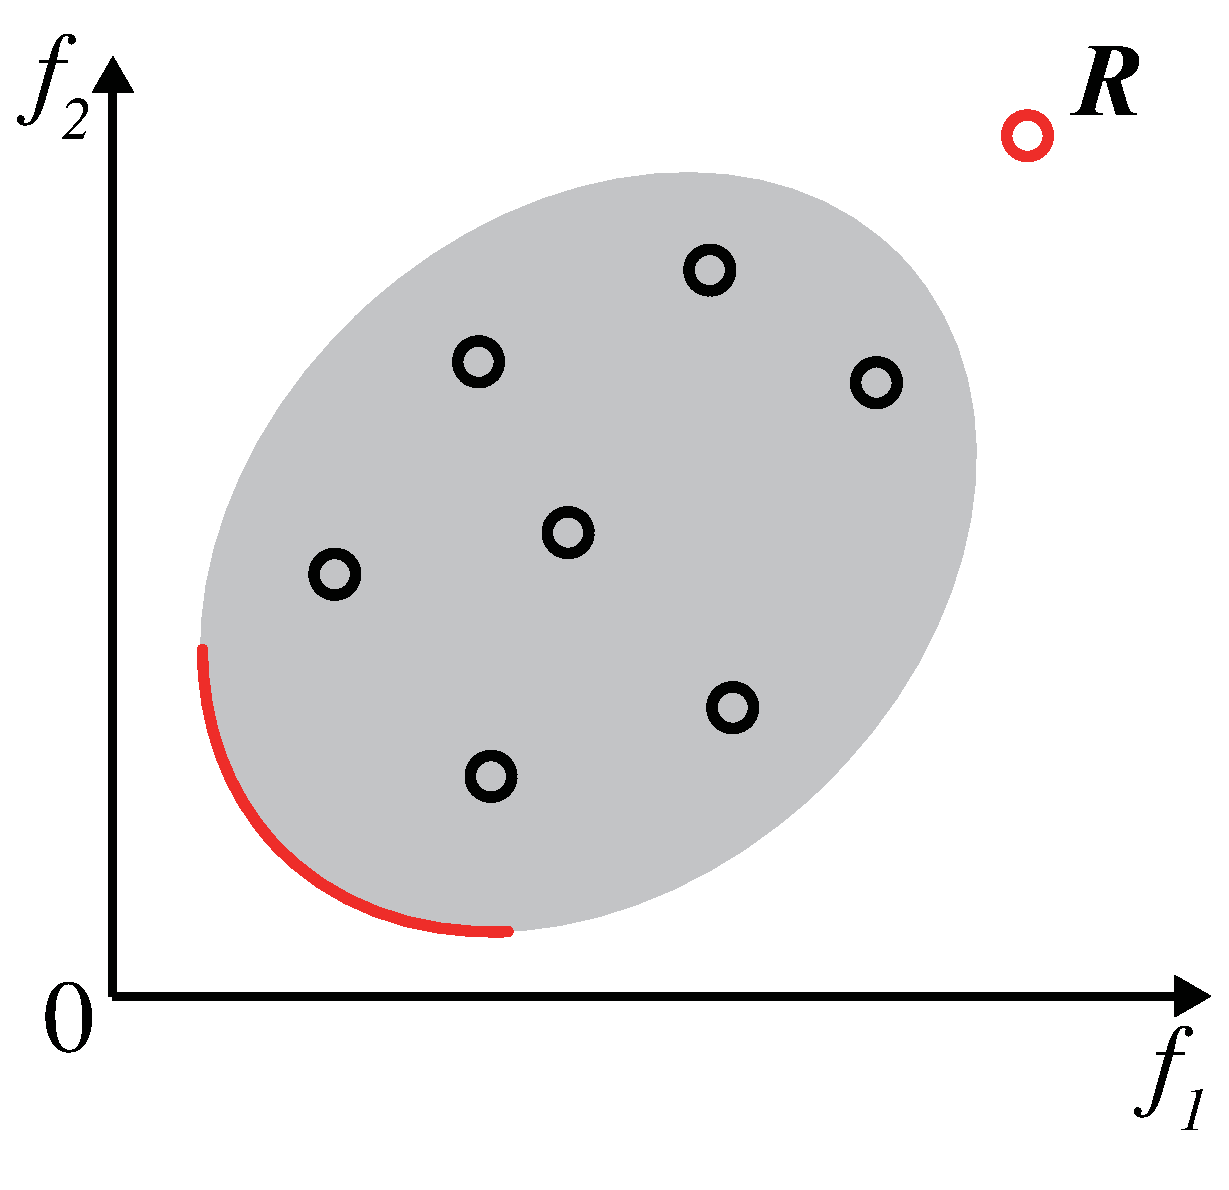
\includegraphics[width=1.5in]{rpa1_1}}\quad
  \subfloat[The final generation.]{\label{rpa1:b}
  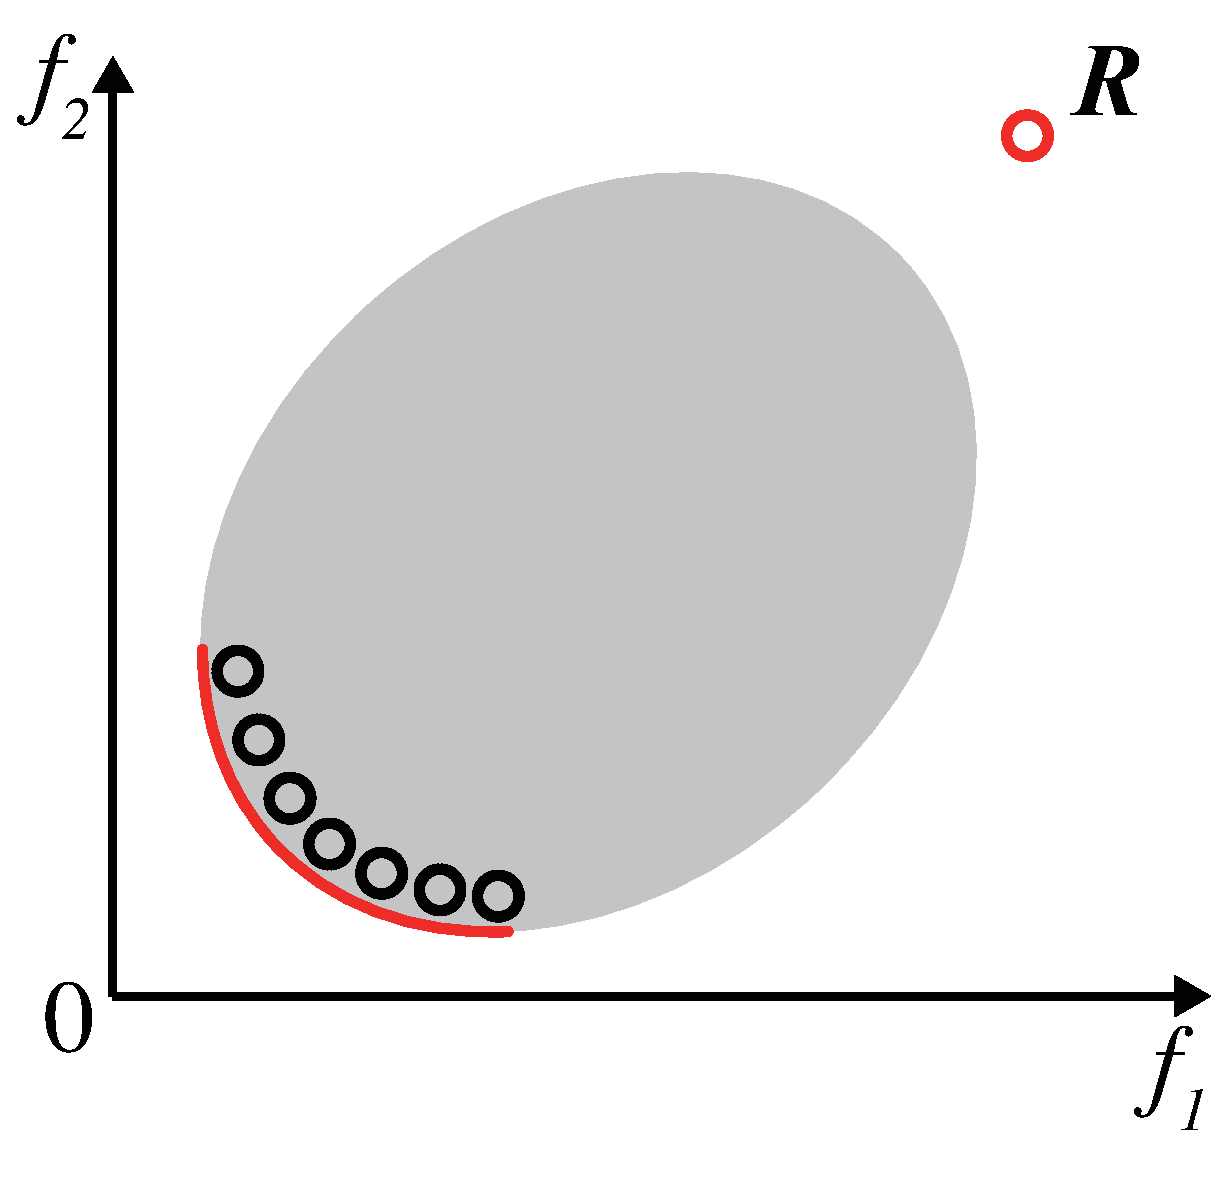
\includegraphics[width=1.5in]{rpa1_2}}\\
  \caption{The reference point is set with a large feasible space.
  The PF can be far away from reference point.
  The gray region shows the feasible region and the red arc is the corresponding PF.
  The red circle $r$ is the reference point calculated by the initial solutions in (\ref{rpa1:a})
  which is randomly generated.
  After some generations, the current solutions reach to the five black circles in (\ref{rpa1:b}), 
  which is far away from the reference point.}
  \label{rpa1}
\end{figure}

There is a big problem when applying this strategy to some problems with special PF shape. 
For example, the inverted-DTLZ1\cite{invertedDTLZ1} has an inverted-triangular PF, 
so many solutions in the final solution set will distribute on the boundary of the PF
(Fig. \ref{rpa2:a})\cite{hisao:RPexplanation, hisao:RPspecify, hisao:dynamic}. 
Although it has no effect on the distributions of solution set 
in triangular PF problems 
(Fig. \ref{rpa2:c} comparing with Fig. \ref{rpa2:d}), 
it is necessary to use a good reference point specification method during the algorithm progress.
The reason is explained in detail in\cite{hisao:RPexplanation}.

\begin{figure}[!t]
  \centering
  \subfloat[The reference point is fixed.]{\label{rpa2:a}
    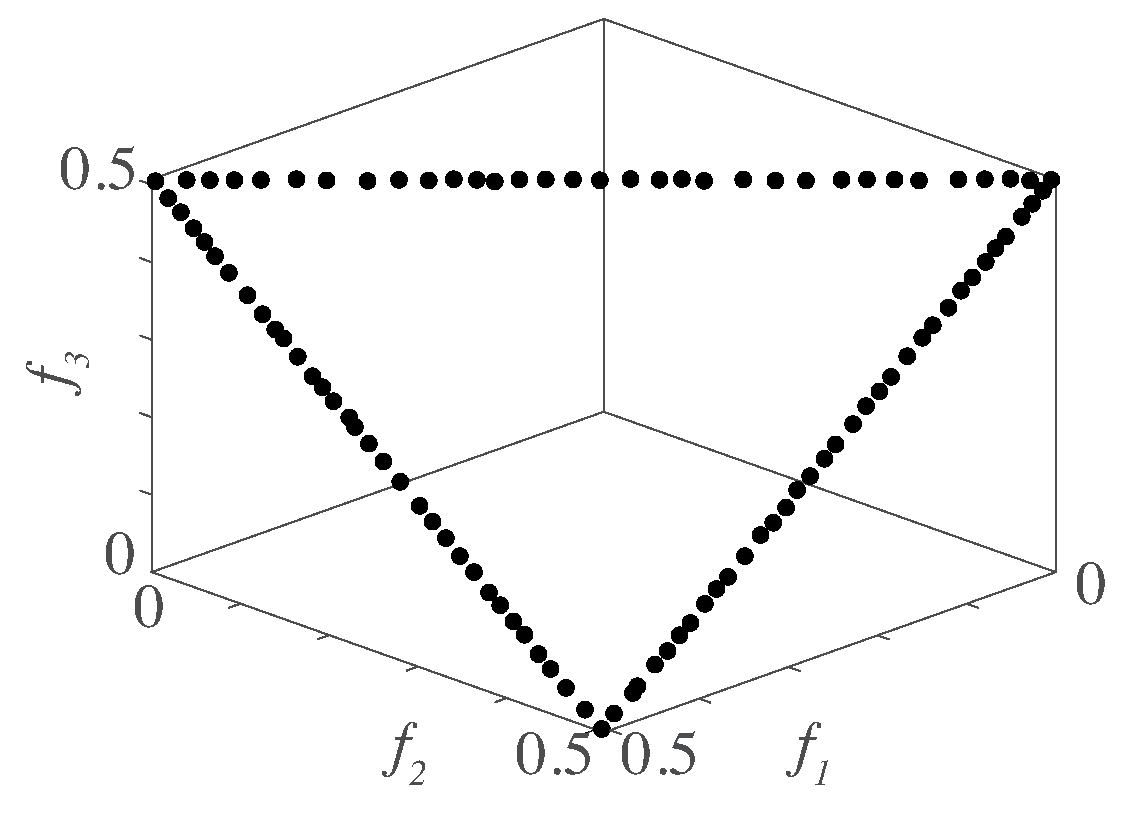
\includegraphics[width=1.5in]{FVEMOA_fixrp_IDTLZ1_evaluation20000_r1__1}}\quad
  \subfloat[The reference point is specified by Eq. (\ref{frpa1}).]{\label{rpa2:b}
    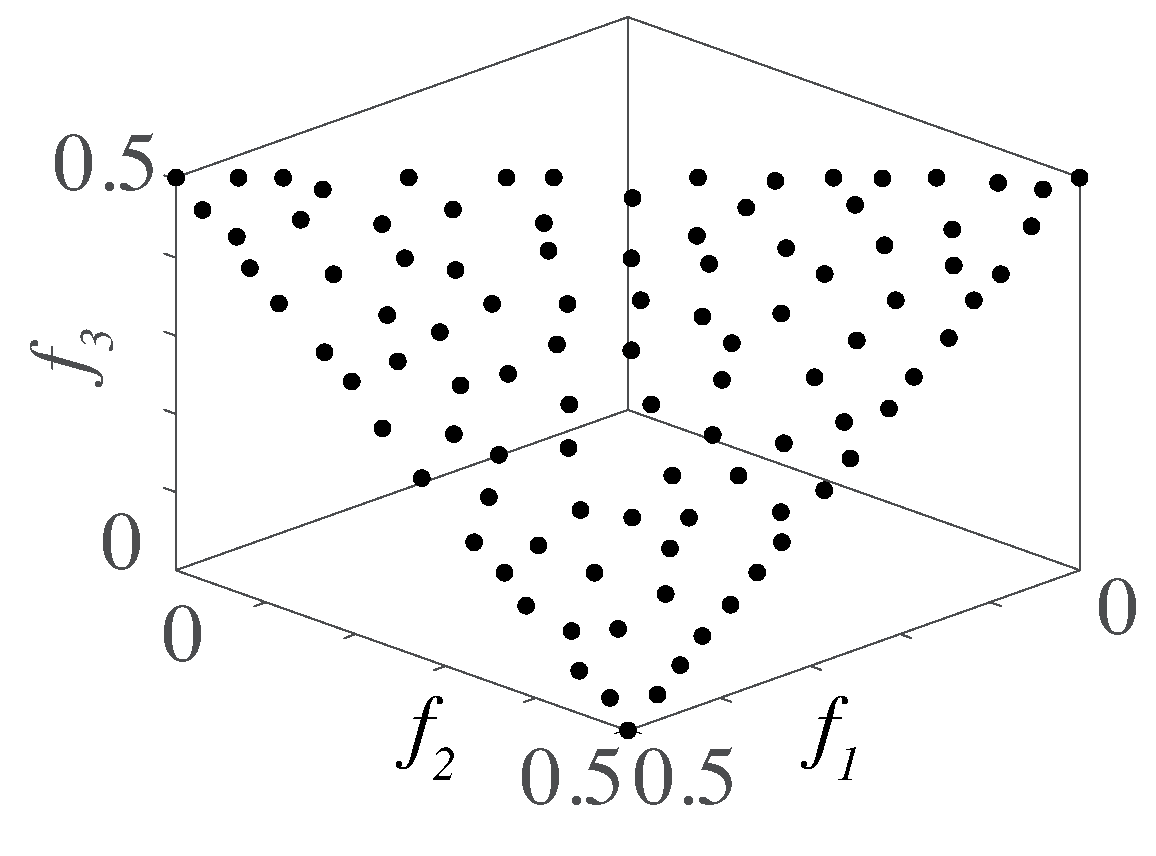
\includegraphics[width=1.5in]{FVEMOA_IDTLZ1_evaluation20000_r1__1}}\\
  \subfloat[The reference point is fixed.]{\label{rpa2:c}
    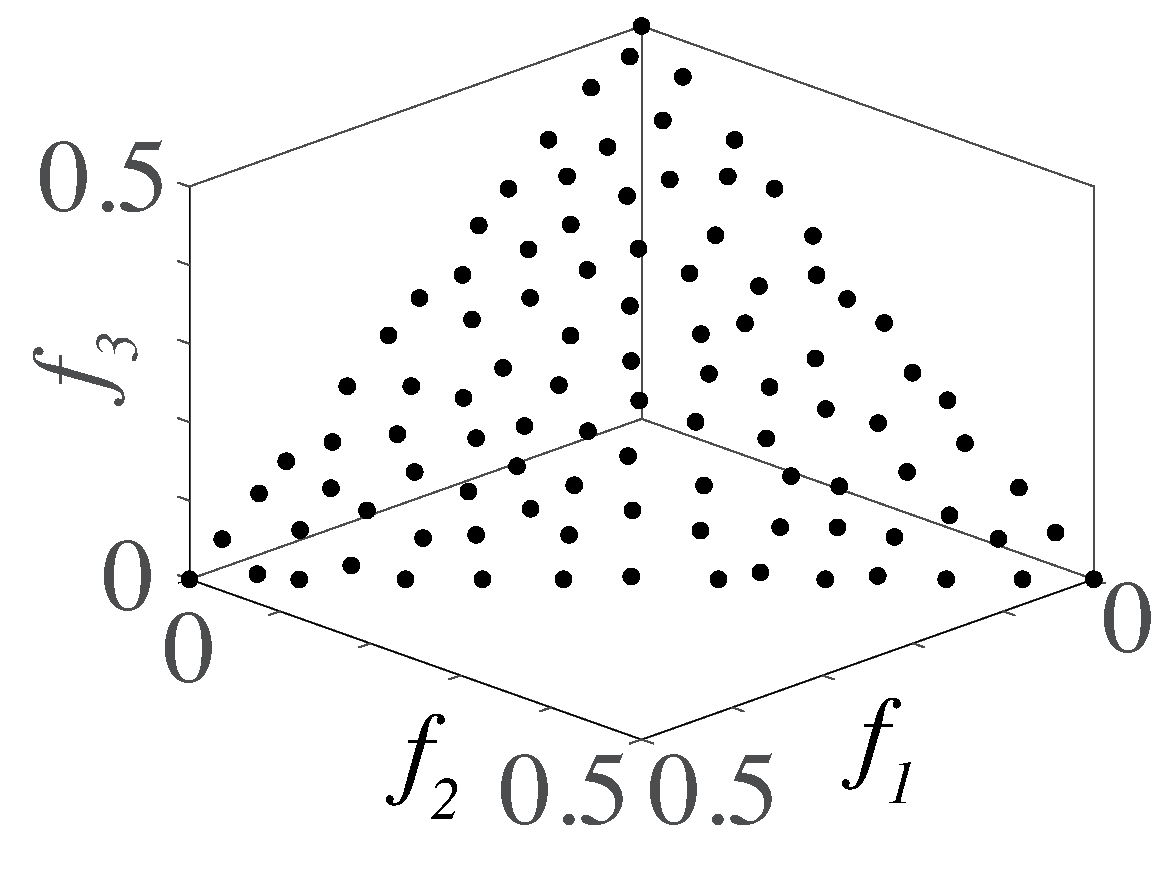
\includegraphics[width=1.5in]{FVEMOA_fixrp_DTLZ1_evaluation20000_r1__1}}\quad
  \subfloat[The reference point is specified by Eq. (\ref{frpa1}).]{\label{rpa2:d}
    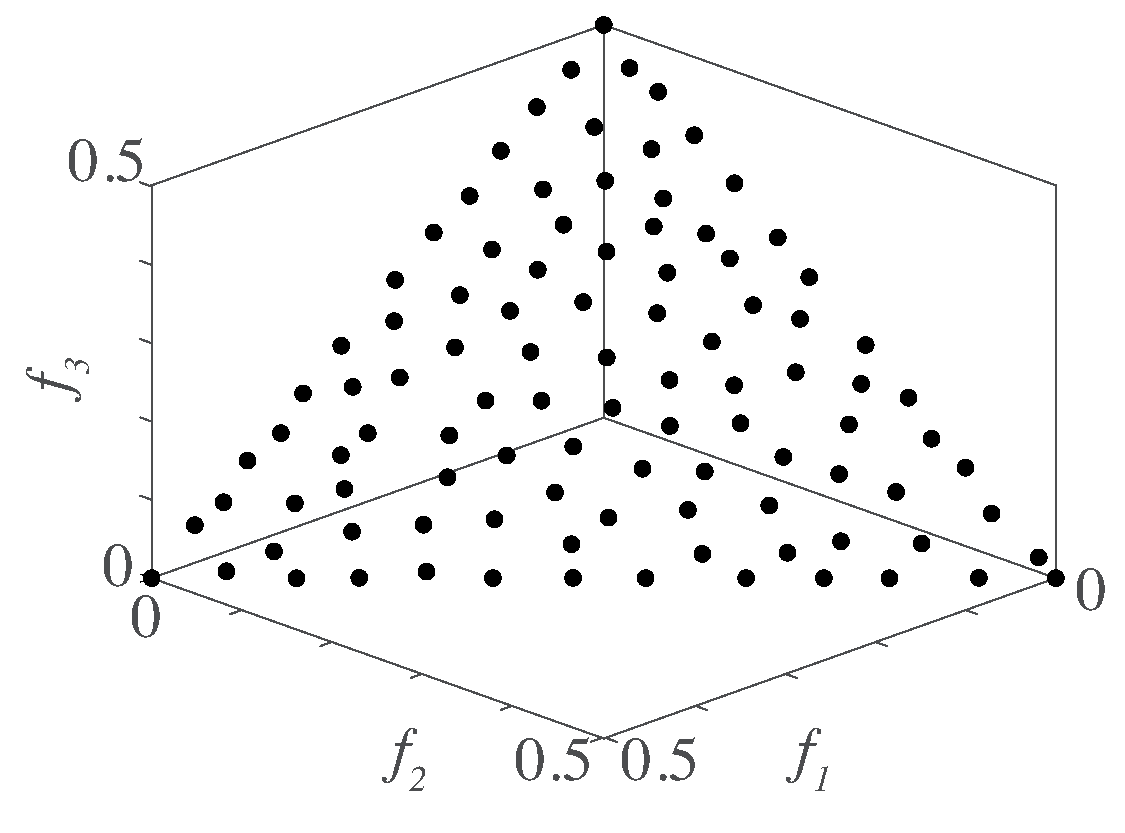
\includegraphics[width=1.5in]{FVEMOA_DTLZ1_evaluation20000_r1__1}}\\
  \caption{The final distribution of solution set in the inverted-DTLZ1(\ref{rpa2:a} and \ref{rpa2:b}) 
  and the DTLZ1 problem(\ref{rpa2:c} and \ref{rpa2:d}).
  The algorithm is SMS-EMOA with population size $= 100$, evaluation number $= 20000$. 
  \ref{rpa2:a} and \ref{rpa2:c}: the reference point is calculated only once at the initial step;
  \ref{rpa2:b} and \ref{rpa2:d}: the reference point is specified by the Eq. (\ref{frpa1}) with $r=1.1$.
  All the solutions in the final distribution are on the boundary of the PF in (\ref{rpa2:a}),
  which shows the bad effect of a faraway reference point
  on the final distribution of inverted-triangular problems.
  This bad effect can not be observed on triangular problems in (\ref{rpa2:c}).
  }
  \label{rpa2}
\end{figure}

\subsection{Original Reference Point Specification}
In the original paper of SMS-EMOA\cite{smsemoa}, 
the reference point is specified as the estimated nadir point increased by $\boldsymbol{1.0}$
(in two-dimension, a sufficiently large reference point is chosen). 
But in current implementation, the following mechanism is always used:
\begin{equation}\label{frpa1}
  \boldsymbol R = r * \boldsymbol N, 
  \boldsymbol R, \boldsymbol N \in \mathbb{R}^m, 
\end{equation}
where $\boldsymbol R$ is the reference point in each generation, 
and $\boldsymbol N$ is the estimated nadir point of the last front of the current population. 
$r$ is specified as 1.1 in PlatEMO\cite{PlatEMO}, a well-known EMO framework. 
The specification of reference point is also one of the important parts in the HV-based algorithm implementation.
In the source code of PlatEMO, the values of $r$ in HV-based algorithms are chosen as follow: 
1.1(SMS-EMOA\cite{smsemoa}) and 1.2(HypE\cite{HypE}). % and 10(FV-EMOA\cite{FVEMOA}). 
When the solutions in the current population are obtained, 
we use HV as the indicator to evaluate the performance of the solution set. 
Then the reference point used to calculate the HV is calculated by the formula above. 
%可以加一个介绍nadir point的图,如果8页不够的话。 !!!!!!!!

However, fixing the $r$ value to 1.1 is not recommended, especially on problems with the inverted-triangular PF
\cite{hisao:RPhowtoSpecify}. 
The research on specifying the value of $r$ is limited, for the reason that, 
the effect of the location of the reference point on the PF 
is not fatal on some benchmark problems, for example, the problems with triangular PF. 

% --------------- reference point specification for optimal distribution ----------------
% 在hisao的paper中指出r = 1+1/H 在一些问题中(平的PF问题)是最优的设置(画出二维三维图for example),
% 提一句 本文主要的研究问题就是平的PF问题
% 即在算法的最后final stage,所有solution都在PF上,r应该设置成1+1/H。
%
\subsection{Reference Point Specification Proposed in \cite{hisao:RPhowtoSpecify}}
In \cite{hisao:RPexplanation, hisao:RPhowtoSpecify, hisao:RPspecify}, the suggested value of $r$ is investigated 
on linear PF problems. 
Specifically, on inverted-triangular problems(inverted-DTLZ1\cite{hisao:RPexplanation} etc.), 
in order to have same HV contribution, 
the interval between two boundary solutions should be the same as that between two inner solutions.
In \cite{hisao:RPhowtoSpecify}, the suggested value of $r$ is:
\begin{equation}\label{eod}
  r=1+\frac{1}{H}.
\end{equation}
$H$ is the number of solutions intervals in 2-dimension 
and the number of intervals on each boundary of PF in many-dimension. 
The idea is inspired from MOEA/D\cite{MOEAD}, in which the $H$ is used for 
generating uniformly distributed weight vectors\cite{hisao:dynamic}. 
Given the population size $\mu$ and dimensionality $m$, the value of $H$ can be calculated by the following formula:
\begin{equation}
  C^{H+m-1}_{m-1} \leq \mu < C^{H+m}_{m-1}.
\end{equation}
In Fig. \ref{dm1:a}, $r=13/12(H=12)$ is the optimal setting for a 91-individual 3-dimensional 
inverted-DTLZ1 problem and a uniform distribution is observed. 
In Fig. \ref{dm1:b} - Fig. \ref{dm1:d}, the inner solutions are decreased and move to 
the boundary of PF with the increasing of $r$. 

\begin{figure}[!t]
  \centering
  \subfloat[$r=13/12$(optimal).]{\label{dm1:a}
    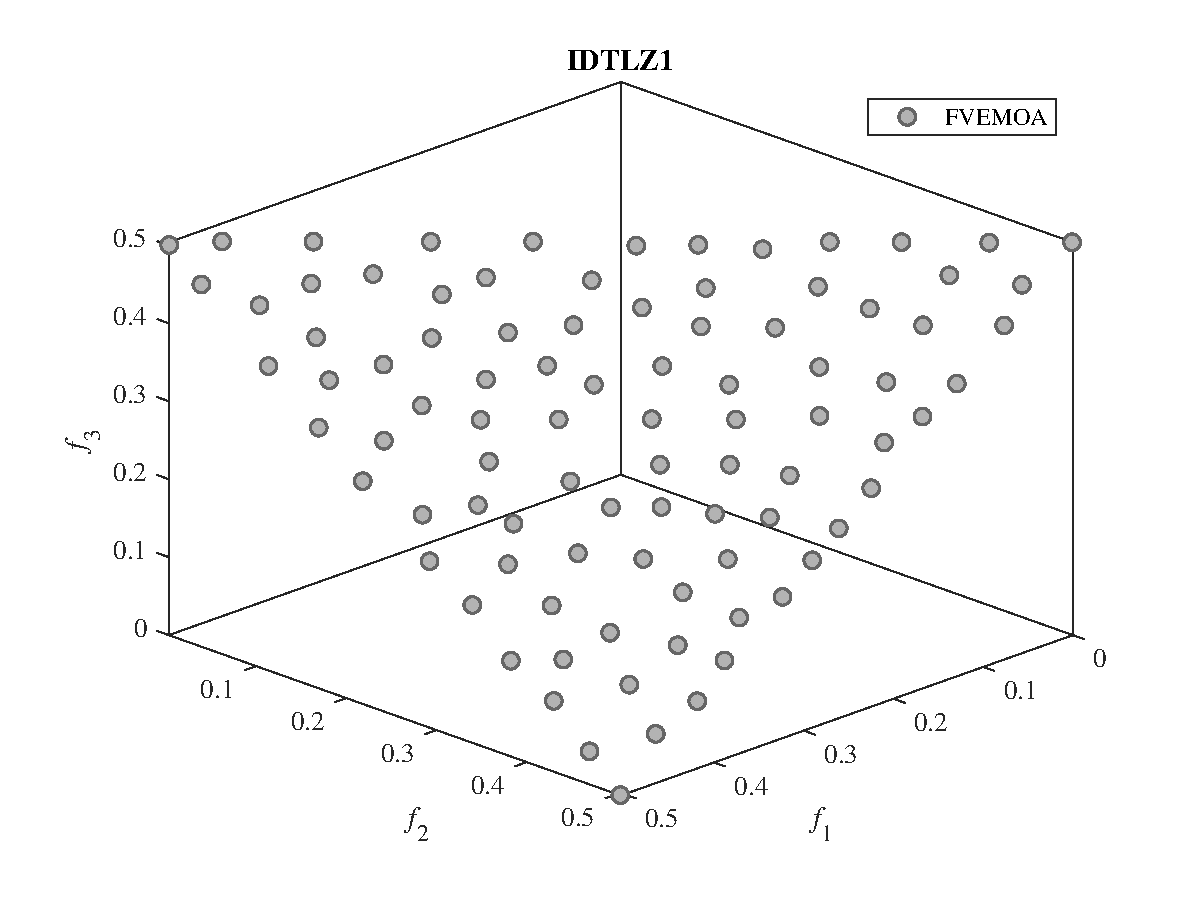
\includegraphics[width=1.5in]{FVEMOA_IDTLZ1_evaluation10000_r13_12_N91}}\quad
  \subfloat[$r=1.5.$]{\label{dm1:b}
    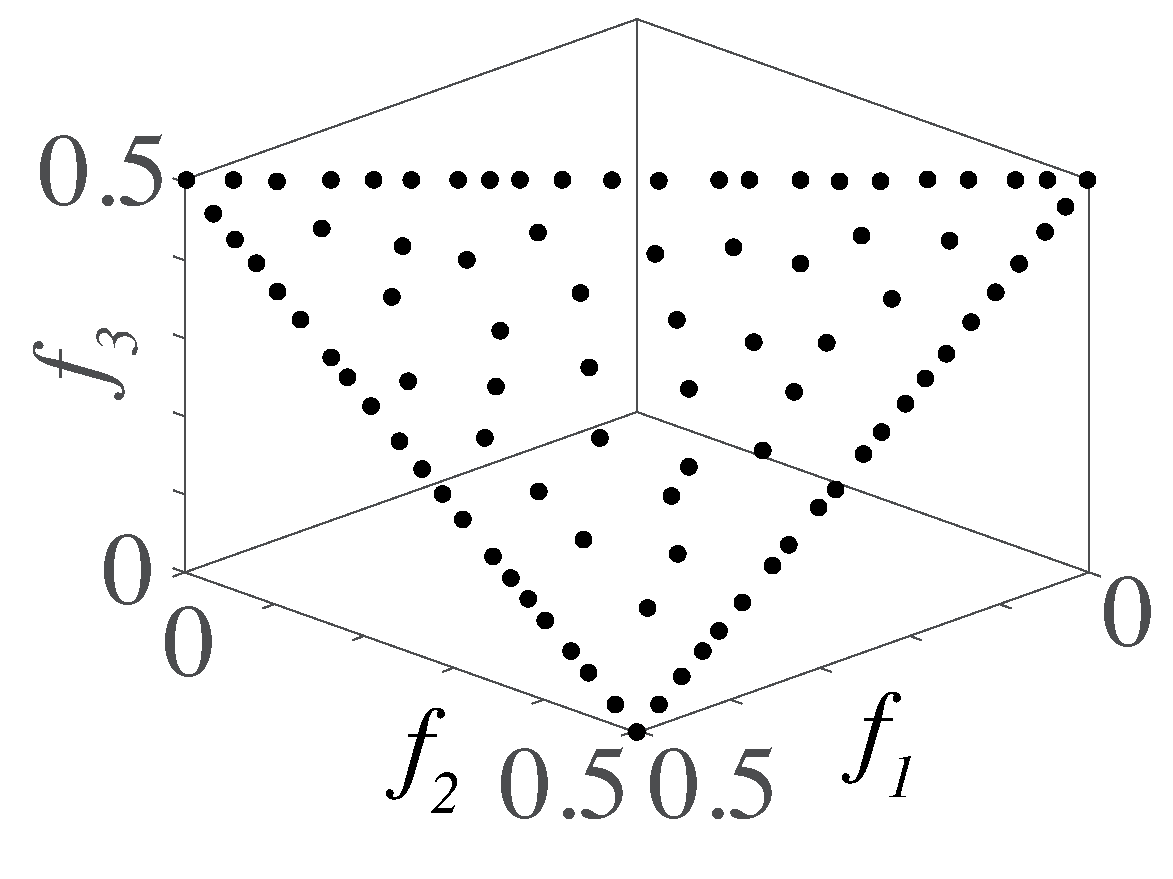
\includegraphics[width=1.5in]{FVEMOA_IDTLZ1_evaluation10000_r1__5_N91}}\\
  \subfloat[$r=2.$]{\label{dm1:c}
    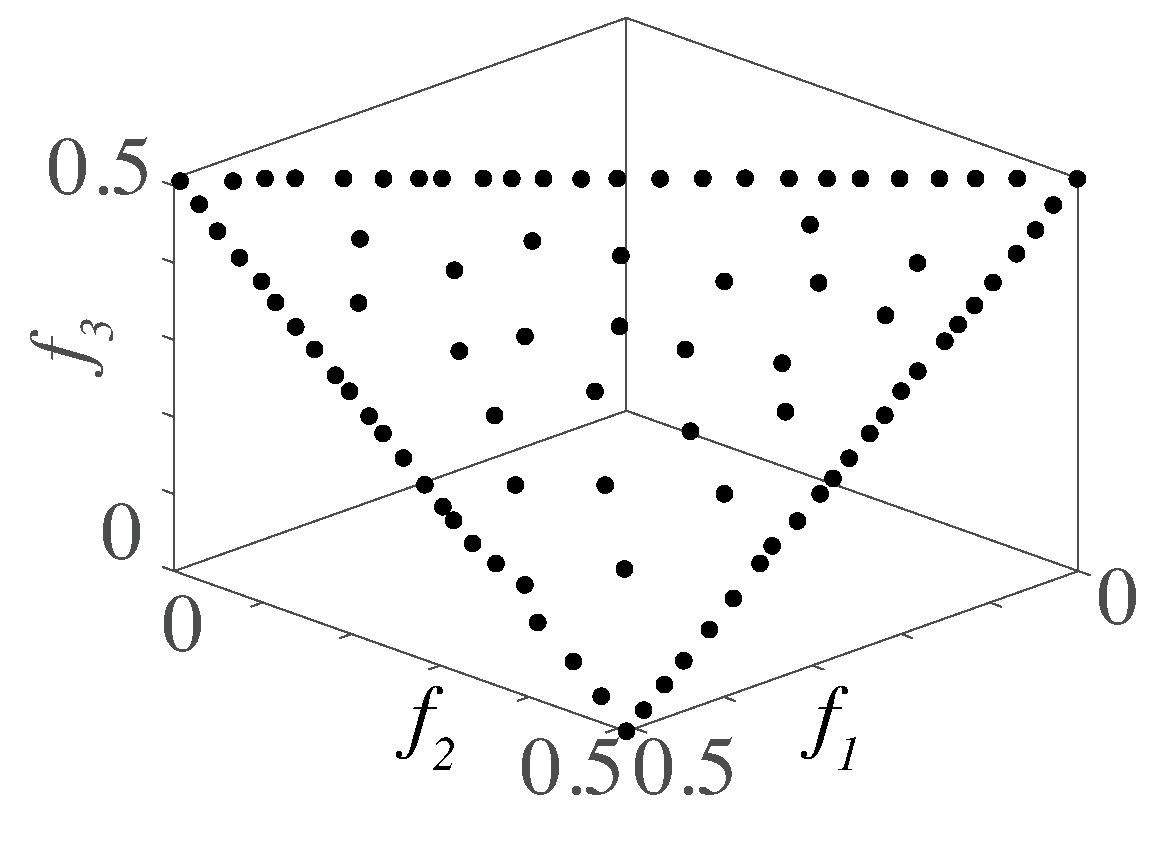
\includegraphics[width=1.5in]{FVEMOA_IDTLZ1_evaluation10000_r2_N91}}\quad
  \subfloat[$r=5.$]{\label{dm1:d}
    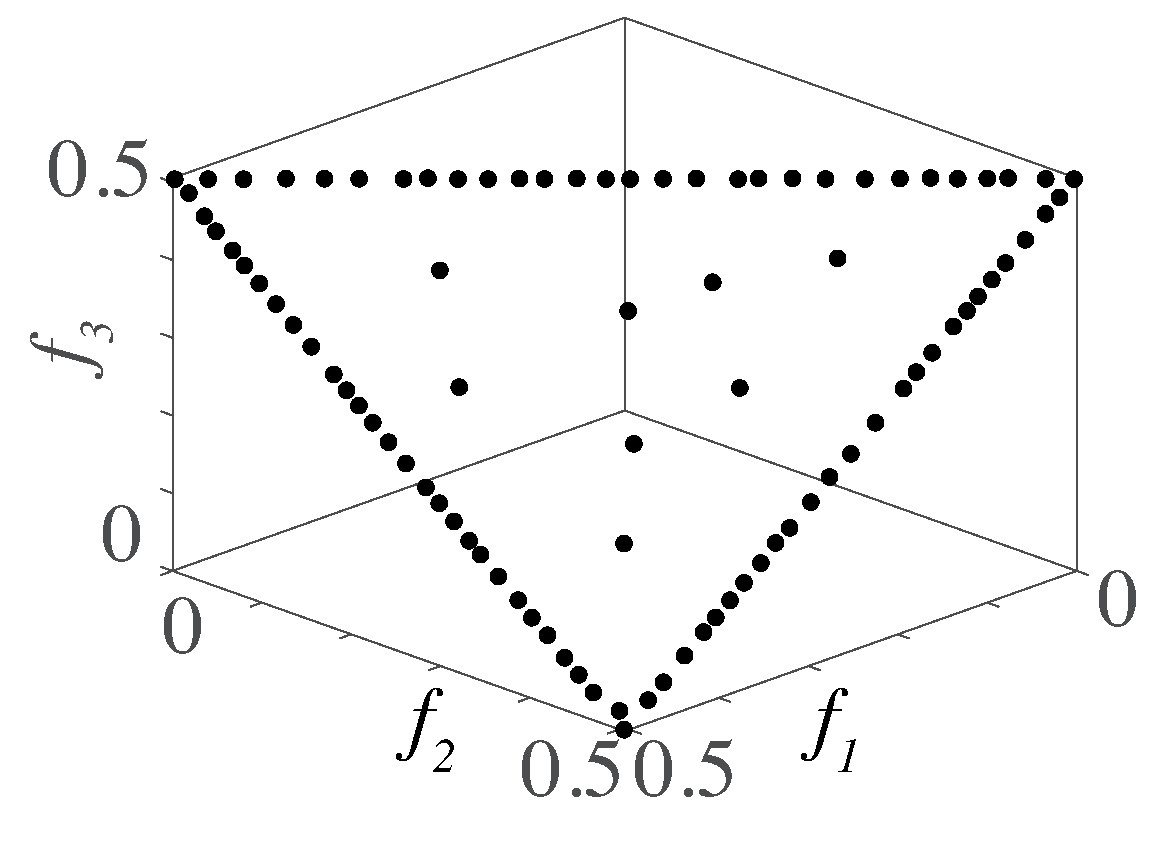
\includegraphics[width=1.5in]{FVEMOA_IDTLZ1_evaluation10000_r5_N91}}\\
  \caption{The final distribution of solution set on the inverted-DTLZ1 problem.
  The algorithm is SMS-EMOA with population size $=91$($H=12$) and evaluation number $=20000$.
  $r=13/12$ is the optimal setting and we observed a evenly distribution in (\ref{dm1:a}).
  As the increasing of $r$, solutions are more likely to be on the boundary
  (\ref{dm1:b}-\ref{dm1:d}). 
  }
  \label{dm1}
\end{figure}

% ----------------------------------- dynamic mechanism ------------------------------------
% 在算法运行的不同时期 early stage;final stage, 为了不同的目的,
% (early stage是convergence, final stage是diversity) r应该设置成不同的值【我的本科毕设和hisao】
% 即 r value 应该是随着算法的进行dynamically设置成不同的值。 
%
% unfortunately 对r的研究太少了, 因为在 benchmark问题上, 特别是正三角 r对PF上的解的影响很小
% 但是实际上 在一些问题上 最后PF上解的分布情况是对r很敏感的【hisao paper里的倒三角和最近点问题】
% 
% \section{Exploration on Reference Point Specification Mechanism in Detail}
Basically, the process of EMOAs can be separated into
two stages:
\subsubsection{Early Stage} In this stage, 
all the solutions are far away from the PF.
The main task is to converge the solutions to the PF.
We also call this stage the convergence stage.
\subsubsection{Final Stage} In this stage,
all the solutions are inside or near the PF. 
So the main task is to make the distribution of solutions more evenly in the PF.
We also call this stage the diversity stage.

% ------------------sub-------------- dynamic mechanism ----------------------------------
% --------------- reference point specification for better searching behavior ------------
% hisao指出如果一直用1+1/H, 在convergence阶段会有不好的 search behavior,因为
% specify 1+1/H in each generation, 在 early generations
% the estimated ideal and nadir points from the nondominated
% solutions in each generation 离PF太远。
% 因此 对于normalization based on the estimated ideal and nadir points 
% often has unexpected bad effects on the search behavior
%
% in early generations, a slightly larger r is suggested in 【hisao和我的本科毕设】
% 大一点的r能够加快convergence 用NHV试试 log(HV)
% (加图 相同的evaluation 一直optimal和一直2 一直2会快点收敛 一个HV 一个NHV, 
% HV表示最后hv差,NHV表示较快到达前沿)
% (图 r越大,收敛越快,从三维开始 画出hv变化斜率图)
% 
\subsection{Specify the Value of $r$ for Better Searching Behavior}
In the early stage, solution set is not close to the PF, which makes the 
estimated ideal and nadir points far away from true ideal and nadir points, for the reason that
they are calculated by current solutions in each generation. 
And considering the problems with 10 objectives, 
if the external solutions have the same HV contribution with the inner solutions, 
the exploration of solutions will be poor. 
As a result, some dimensionalities of solutions will be missing and the breadth-diversity\cite{DtA} will be poor. 
An example is given in Fig. \ref{nud}. 
\begin{figure}[!t]
  \centering
  \subfloat[$r=10$.]{\label{nud:a}
    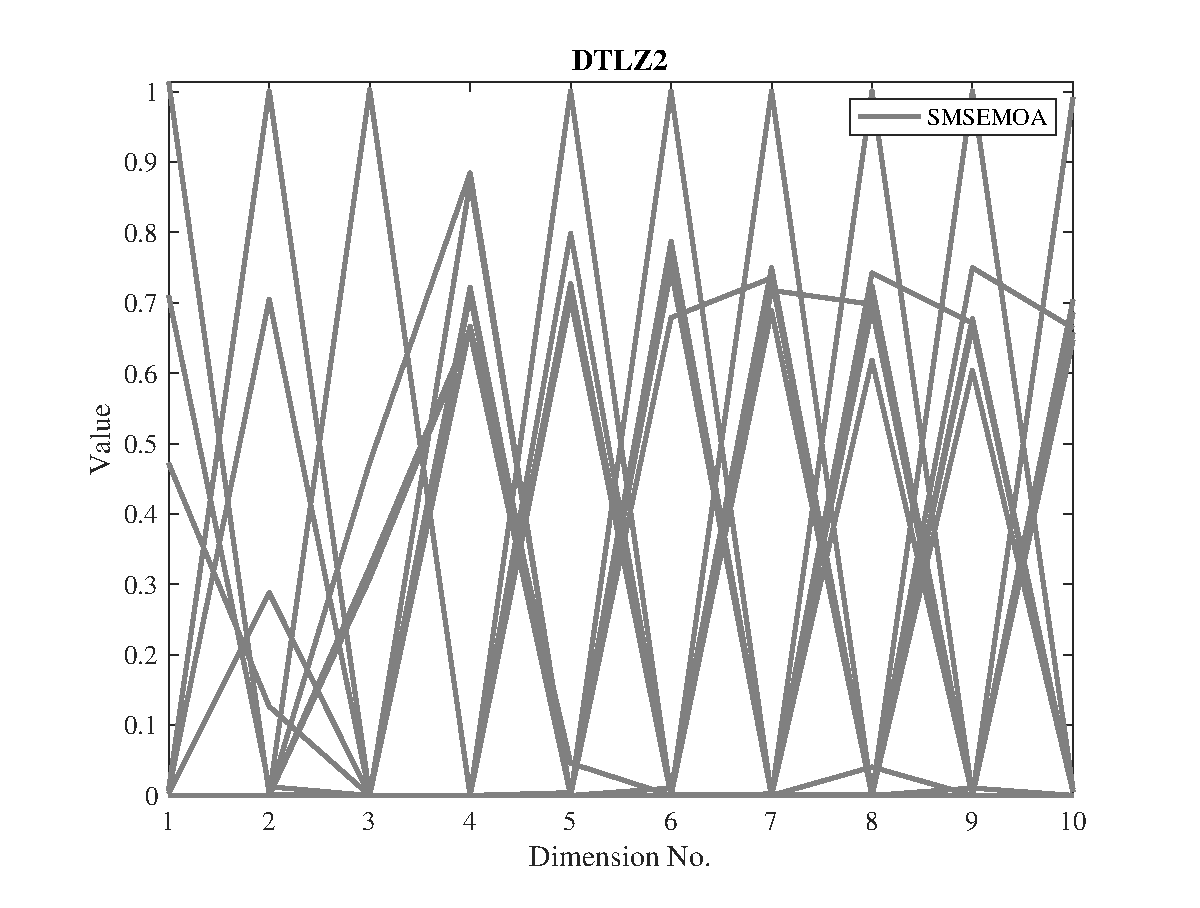
\includegraphics[width=1.5in]{SMSEMOA_DTLZ2_e10000_r10}}\quad
  \subfloat[$r=2$(optimal).]{\label{nud:b}
    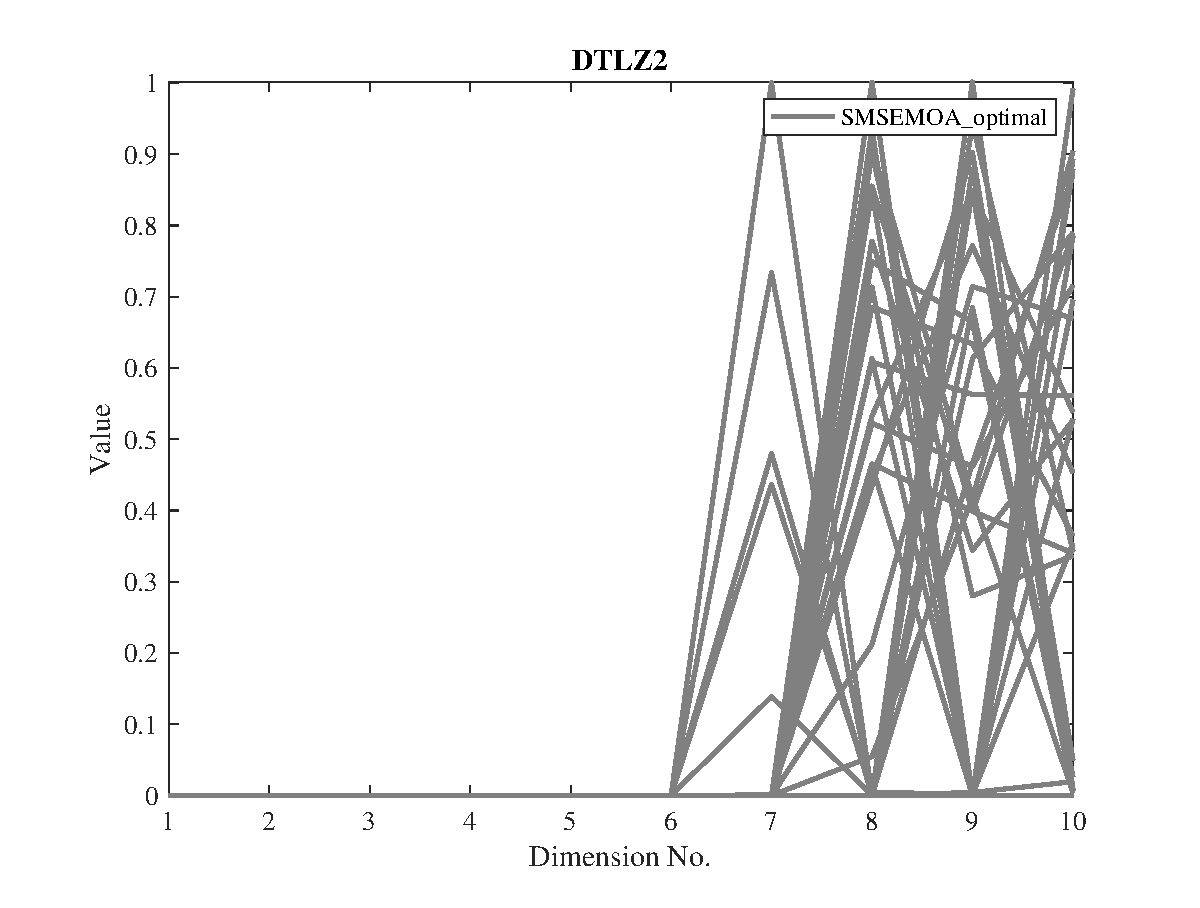
\includegraphics[width=1.5in]{SMSEMOA_optimal_DTLZ2_e10000}}\\
  \caption{
    The final distribution of SMS-EMOA on 10-objective DTLZ2 problems with different settings of $r$. 
    The population number is 30($H=1$), total evaluation number is 10000.
  }
  \label{nud}
\end{figure} 
The first 6 dimensionalities are all 0 for the solutions obtained by SMS-EMOA on 10-objective DTLZ2 problems(Fig. \ref{nud:b}). 
In \cite{hisao:dynamic}, a larger value of $r$ than $1+1/H$ is suggested in the early stage. 

\subsection{Specify the Value of $r$ for Uniform Distribution}
When algorithm reaches the final stage, all solutions are near the PF, $r$ should
be specified as $1+1/H$, as in Eq. (\ref{eod}), 
in order to get an uniform solutions distribution. 
That is, $r(T)=1+1/H$. 
On inverted-triangular problems, the distribution of solutions on PF
strongly depends on the value of $r$ (as shown in Fig. \ref{dm1}). 

The sensitivity of the value of $r$ on the solutions distribution is also observed on some real-world problems,
for example, distance minimization problems. 
This observation shows the potential use of the dynamical reference point specification\cite{hisao:dynamic}.

\section{Dynamic Reference Point Specification Mechanism}
For different purposes in the two stages, the $r$ should be treated differently\cite{hisao:dynamic}. 
Not only the reference point but also the value of $r$ 
needs to be adapted in each iteration of the algorithm. 
This is called dynamical reference point specification. 
Based on the Eq. (\ref{frpa1}), 
we define the dynamic reference point specification as:
\begin{equation}\label{f2}
  \boldsymbol R = r(t) * \boldsymbol N, 
  \boldsymbol R, \boldsymbol N \in \mathbb{R}^m, t=0,1,\dots,T,
\end{equation}
where $T$ is the total number of generations, and $r=r(t)$ is a function of the current generation $t$.
The value of $r$ is adapted during the process of the algorithm. 

% ------------------------- linearly decrease mechanism --------------------------
% so r从2到1+1/H 很必要 之前介绍过 但是怎么变化 没有一个特别好的idea outperform the others
% hisao的paper,提到一种linearly decrease 机制 就是从2到1+1/H线性下降 这是一种简单又实用的idea
% 图在下一个section画。
% 接下来本文介绍一种基于weak convergence detection criterion, 在一些限制条件下outperform线性机制。
% 
\subsection{Linearly Decreasing Mechanism Proposed in \cite{hisao:dynamic}} 
Based on the theory above, $r$ is suggested to be specified dynamically at different stages of
the algorithm(at early stage, a larger $r$ is chosen; at final stage, $r=1+1/H$ is chosen).
But unfortunately, there is no best mechanism on how to specify the value of $r$ dynamically
that outperforming the others in all problems and all experiment settings. One mechanism may be the best
when working on some specific experiment conditions, but may not be good on other conditions. 

In \cite{hisao:dynamic}, a linearly decreasing mechanism has been proposed:
\begin{equation}\label{eldm1}
  r(t)=r_{Initial}\frac{(T-t)}{T}+(1+1/H)\frac{t}{T}, t=0,1,\dots,T,
\end{equation}
where $T$ is the total number of generations, and $r_{Initial}$ is the initial value of $r$,
which is larger than $1+1/H$. 
It is a simple and practical mechanism. In (\ref{eldm1}), the value of $r$ starts from $r_{Initial}$,
then gradually decreases to the suggested value in a linearly decreasing process. 

In the next section, another dynamic mechanism based on weak convergence detection criterion is proposed. 
We show that it outperforms simple linearly decreasing mechanism on some specific problems. 


% -------------------------------- new dynamic mechanism ------------------------------------
% 本文介绍一种基于weak convergence detection criterion的 new mechanism
% 当 检测到convergence 就把r从2变成optimal 
% (画 r 随 evaluation变化图 就是z字型那个 和线性机制一起画)
% 
\subsection{A New Dynamic Reference Point Specification Mechanism}
In this section,
we will introduce a new mechanism that uses a weak convergence detection criterion to 
decide whether to change the value of $r$ from $r_{Initial}$ to $1+1/H$. 

As we have explained before, 
a larger $r$ is suggested at the early stage of the algorithms. 
But for good diversity at the final stage,
it is needed to set $r$ to its optimal value ($1+1/H$). 
For this purpose, it is necessary to detect whether the algorithm is converged. 
If solutions are all close to the PF, 
we change the value of $r$ to $r_{Optimal}$; otherwise, we set value of $r$ to 
$r_{Initial}$. The mechanism is shown below:
\begin{equation}\label{endm1}
  r(t)=
  \begin{cases}
    r_{Initial}, t<t_{Converged}\\
    1+1/H, t \ge t_{Converged} 
  \end{cases}
  t=0,1,\dots,T.
\end{equation}
$r(t)$ equals to $r_{Initial}$ before reaching the converged generation $t_{Converged}$, 
and changes to $1+1/H$ after $t_{Converged}$. 
$t_{Converged}$ is determined by a weak convergence detection criterion. 

% ---------------sub-------------- new dynamic mechanism ------------------------------------
% ----------------------------- weak convergence detection ----------------------------------
% consider some convergence detection paper【各种 convergence detection paper】
% convergence detection一般用各种各样的indicator【各种paper】
% 总结特点:用indicator list的太花时间;精确的收敛检测
%
% 准则:
% convergence detection 不应该花太多时间,并不需要太准  用 subsubsection
% 需要寻找一种不需要花太多计算量的 weak criterion
% 【一些paper】indicator based algorithm用indicator
% for us,it seems to be a good idea to use HV 作为indicator,however
% 但是程序运行过程中 hv的reference point 一直在变,所以不同generations没有可比性
% (画一张算法运行过程中用的hv的图)
%
% estimated nadir point 会越来越接近PF, 并且当solutions reach to PF后 NaidrP stagnation
% (画 HV和bsf ln(nadir point) mean的图 最好用MaF1的 可能平滑些)表示它们同时期变化。 
% good idea to use ln(nadir point) mean作为判断解是否reach to PF 的 indicator
% 一篇论文(Introducing a Robust and Efficient Stopping Criterion for MOEAs)实现了
% the Least Squares Stopping Criterion for convergence detection 
% when indicator has reached a stagnation situation, stop
% 用一种简单并且直观SIMPLE INTUITIVE 的方式 就是剩余价值和线性回归斜率 below thresholds
% 介绍机制 线性计算公式
% 画上图(ln np mean)的b随evaluation变化图
% for nadir point, 经过我们的实验 10^-5是个好threshold
%
Various indicators including convergence detection indicators that are used to detect the stagnation 
have been proposed in the literature\cite{convergenceDetection:1, convergenceDetection:LSSC, 
convergenceDetection:OCD, convergenceDetection:OFCDandOCD, convergenceDetection:convergenceMetric, 
convergenceDetection:maxCD, convergenceDetection:online}. 
They focus on the accuracy of convergence, which is not the purpose in our approach for 
the reason that after algorithm converged, we still need some generations in order to
get even distribution of solution set. 
We summarize our weak convergence detection criterion as follow:
\subsubsection{inaccuracy} It is not necessary to have an accurate convergence detection. 
The convergence can be reported if current solutions are close to the PF.
In other words, the estimated ideal and nadir points based on the current solutions
are close to the true ideal and nadir points. 
\subsubsection{saving time} We should not spend too much time in convergence detection
for the reason that the state-of-the-art HV-based algorithms such as SMS-EMOA and HypE, 
are time-consuming when the dimension is very high. 

We are discussing the effect of reference points in calculating HV. It seems to be a good
idea to use HV as our convergence detection indicator as we have calculated 
HV in each generation in SMS-EMOA. 
But during the process of algorithm, the reference point is calculated by Eq. (\ref{frpa1}), 
which means that they are different among generations. 
So, we can not simply compare HV calculated in algorithm among different generations. 

We are trying on some other good indicators satisfying our convergence detection criterions. 
Fig. \ref{wcd1} shows the change of HV and nadir point on SMS-EMOA  
with 3-objective inverted-DTLZ1 problem.
When current solutions are close to the PF, the estimated nadir point of current solutions is close 
to the true nadir points. 
\begin{figure}[!t]
  \centering
    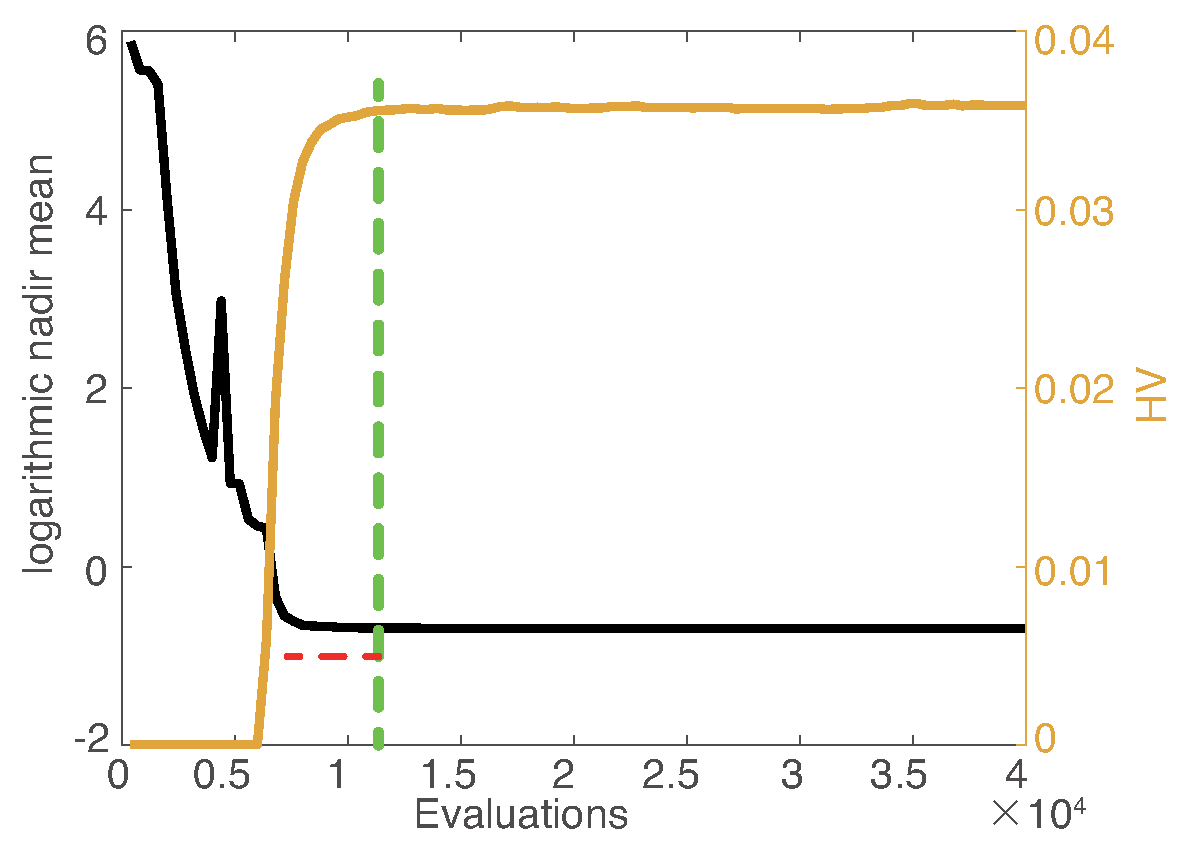
\includegraphics[width=\columnwidth]{FVEMOA_IDTLZ1_M3_nadir_1}
  \caption{Example of nadir point and HV value on 3-objective inverted-DTLZ1 problem
  with SMS-EMOA algorithm.
  The yellow curve is the change of HV 
  while the black curve is the change of the logarithmic nadir point.
  The green dotted line shows the convergence detection 
  and the red dotted line shows the considered window for evaluated number $t_{Converged}$. 
  }
  \label{wcd1}
\end{figure}
This implies that the estimated nadir point can be a good indicator for our purpose. 
But for some problems with a large feasible region, 
the moving distance of the estimated nadir point in the early generations is larger than that near convergence.
So we consider the logarithm. And considering the possible bad variance of the indicator, 
finally, we use the best logarithmic nadir point so-far as our indicator. More specifically,
for a minimization problem, we consider the indicator $I$ as follows:
\begin{equation}\begin{aligned}\label{ewcd1}
  \boldsymbol{N_{t}} &= [f_{t1},f_{t2},\dots,f_{tm}]^\top \in \mathbb{R}^m ,\\
  I_{0} &= \frac{1}{m} \sum_{i=1}^{m}lnf_{0i},\\
  I_{t} &= min(I_{t-1},\frac{1}{m} \sum_{i=1}^{m}lnf_{ti}),
  t = 1,2,\dots,T,
\end{aligned}
\end{equation}
where $T$ is the total number of generations, 
$\boldsymbol{N_{t}}$ is the estimated nadir point at the $t^{th}$ generation with $m$ objectives: $f_{t1},f_{t2},\dots,f_{tm}$. 
$I_0$ is the initial indicator calculated by the initial population.
And $I_t$ is the minimum value before the $t^{th}$ generation (including the $t^{th}$ generation). 

After choosing the indicator, the next step is to detect the stagnation of the indicator.
We use a basic linear regression method called Simple Least Squares\cite{SimpleLeastSquares} with a
simple least squares convergence detection strategy introduced in \cite{convergenceDetection:LSSC}.
If the absolute value of the slope of the indicator is below a threshold, the convergence is reported.
Briefly speaking, for a simple linear regression $I(t)=a+bt$, 
the intercept $a$ and slope $b$ of the $t^{th}$ generation can be calculated 
with the following matrix-based formula:
\begin{equation}\label{elr1}
  \left[
    \begin{matrix}
      a \\
      b
    \end{matrix}
  \right]
  = 
  \left[
    \begin{matrix}
      \sum t_i^2 & \sum t_i \\
      \sum t_i   & w\_ l 
    \end{matrix}
  \right]^{-1}
  *
  \left[
    \begin{matrix}
      \sum t_i * I_{t_i} \\
      \sum I_{t_i} 
    \end{matrix}
  \right]
\end{equation}
where $w\_ l$ is the length of the chosen window
(in the example of Fig. \ref{wcd1}, the chosen window for $t_{Converged}$ is represented with the red dotted line), 
and $t_i$ is the evaluated number in the chosen window.
The value of slope $b$ is shown in Fig. \ref{wcd2} 
(Note that the value in the first $w\_ l$ evaluations is 0, 
and we should not consider the first $w\_ l$ evaluations). 
\begin{figure}[!t]
  \centering
    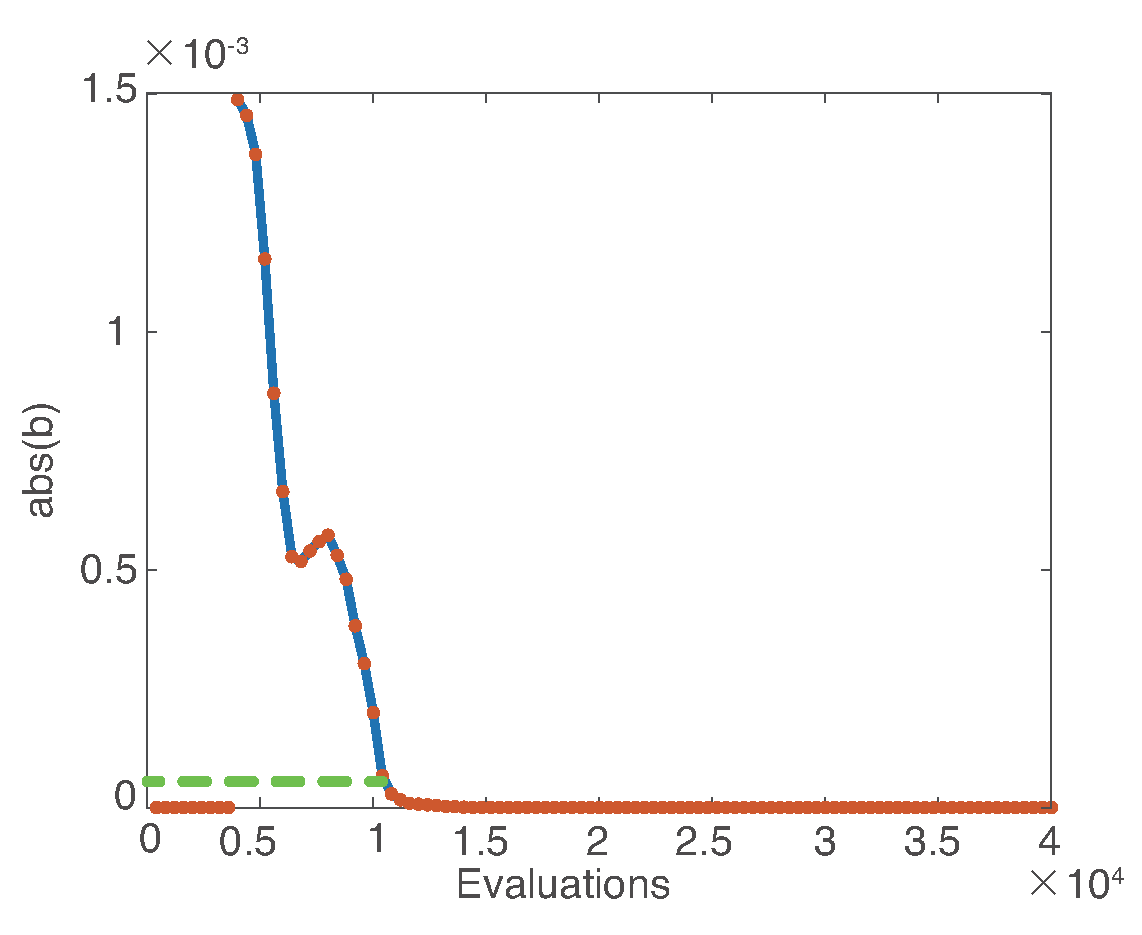
\includegraphics[width=\columnwidth]{FVEMOA_IDTLZ1_M3_nadir_2}
  \caption{Example of $\lvert b\rvert$ on inverted-DTLZ1 3-dimension problem
  (window size = $4000$ evaluations with population size = $100$).
  The green dotted line shows the threshold.
  }
  \label{wcd2}
\end{figure}

With the above Eq. (\ref{elr1}), we report the convergence if the following
formula holds:
\begin{equation}\label{elr2}
  \lvert b \rvert < thres. 
\end{equation}
The value of $t_{Converged}$ equals to $t$ when convergence is detected. 
The whole process of weak convergence detection is also clearly described in Algorithm \ref{alg:wcd}. 
If Algorithm \ref{alg:wcd} return True, we report the convergence, vice versa. 
The choice of the $thres$ value is trivial 
as the report ahead or delay is not fatal to the algorithm or to the final solution set.
We choose $thres$ value as $10^{-5}$ after some experimental computation with 
the window size $w\_ l = 4000$. 
If we do not change the window size, 
this threshold can be applied to other problems or other HV-based algorithms
because of a weak convergence detection purpose.

\begin{algorithm}
  \caption{Weak Convergence Detection}
  \label{alg:wcd}
  \begin{algorithmic}
  \REQUIRE ~~\\
    $w\_l$, $//$ Window size.\\
    $\boldsymbol{s_{t}}$, $//$ Solution set when evaluaiton number is $t$.\\
    $\boldsymbol I = [I_{0},I_{1},\dots,I_{t-1}]^\top$, $//$ Store indicator values. \\
    $thres$, $//$ The chosen threshold for slope. \\ 
  \ENSURE ~~\\
    Calculate nadir point $\boldsymbol{N_{t}}$ of $\boldsymbol{s_{t}}$; \\
    Calculate indicator $I_{t}$; $//$ By Eq. (\ref{ewcd1}). \\
    $\boldsymbol I \gets \boldsymbol I \cup I_{t}$; \\
    \IF{$t \ge w\_l$} 
    \STATE Calculate $b$; $//$ By Eq. (\ref{elr1}).
      \IF{$\lvert b\rvert < thres$}
      \STATE Return True;
      \ENDIF
    \ENDIF
    \STATE Return False;
  \end{algorithmic}
\end{algorithm}
% -------------------------------- Computational Experiments ------------------------------------
% 为了直观的表现dynamic reference point adaptation的优势,
% 算法 sets 我们选用了什么,简单介绍
% 我们选用了test problem:DTLZ1, C1_DTLZ1,IDTLZ1,MaF1 分别介绍
% 维度选择了 3,5,8,10维 为了表现在multi 和 many上的不同
% 
% compare this mechanism with the linearly decrease mechanism
% 
% 要验证 10^-5 是不是一个好的threshold 画出不同维度 当检测到收敛的solutions图,确认检测到不变的时候确实收敛
%
\section{Computational Experiments}
\subsection{Experimental Settings}
To clearly represent the superiority of dynamically reference point specification 
and to ease the comparison process of two different dynamic mechanisms
(linearly decreasing mechanism and weak convergence detection mechanism), 
the mechanisms are tested with the state-of-the-art algorithm SMS-EMOA\cite{smsemoa}.
The test problems include: 
DTLZ\cite{DTLZ}, WFG\cite{WFG}, their minus-versions\cite{minusTestProblem} 
and a multi-objective distance minimization problem(MPDMP)\cite{dmp}.
We test all the problems with 10 objectives. 
All the code in this section is implemented in PlatEMO framework\cite{PlatEMO} 
with the following settings:

Population size: 30 ($H=1$), 

Total evaluation number: 100,000 solution evaluations,

Initial value of $r$ $(r_{Initial})$: 10.

Crossover: simulated binary crossover (probability: 1.0),

Mutation: polynomial (probability: $1/D$),

Number of decision variables $D$:

$\qquad 14$ (DTLZ1 and minus-DTLZ1),

$\qquad 2$ (MPDMP),

$\qquad 19$ (other problems),

Distribution index in Crossover and Mutation: 20, 

Number of runs: 20 runs.

% ---------------sub-------------- Computational Experiments ------------------------------------
% ----------------------------- Computational Results ----------------------------------
% 
\subsection{Computational Results}

\begin{table*}[!t]\footnotesize
  \caption{HV mean and standard deviation over 20 independent runs for DTLZ and WFG problems.}
  \label{table_tri}
  \centering
  \begin{tabular}{ccccccc}
    \toprule
    Problem&$M$&$D$&SMS-EMOA-10&SMS-EMOA-Opt&SMS-EMOA-LD&SMS-EMOA-CD\\ 
    \midrule
    \multirow{1}{*}{DTLZ1}&10&14&6.8448e-1 (4.61e-1) $\approx$&\hl{2.0261e-1 (2.23e-1) $-$}&\semitextbf{8.8369e-1 (2.00e-1) $\approx$}&6.9062e-1 (3.95e-1)\\
    \multirow{1}{*}{DTLZ2}&10&19&\semitextbf{1.0234e+3 (4.72e-1) $\approx$}&\hl{9.9315e+2 (3.94e+1) $-$}&1.0234e+3 (7.28e-1) $\approx$&1.0184e+3 (1.85e+1)\\
    \multirow{1}{*}{DTLZ3}&10&19&\hl{0.0000e+0 (0.00e+0) $\approx$}&\semitextbf{1.9068e+1 (8.53e+1) $\approx$}&0.0000e+0 (0.00e+0) $\approx$&0.0000e+0 (0.00e+0)\\
    \multirow{1}{*}{DTLZ4}&10&19&\semitextbf{8.0029e+2 (2.21e+2) $\approx$}&\hl{5.2691e+2 (1.79e+2) $-$}&6.6262e+2 (2.17e+2) $\approx$&7.2840e+2 (2.26e+2)\\
    \hline
    \multirow{1}{*}{WFG1}&10&19&2.2025e+12 (2.55e+11) $\approx$&2.2597e+12 (2.64e+11) $\approx$&\hl{2.2005e+12 (1.81e+11) $\approx$}&\semitextbf{2.2601e+12 (3.42e+11)}\\
    \multirow{1}{*}{WFG2}&10&19&\semitextbf{3.3604e+12 (2.92e+10) $\approx$}&3.3493e+12 (2.39e+10) $+$&3.3487e+12 (7.64e+10) $\approx$&\hl{3.3420e+12 (8.46e+10)}\\
    \multirow{1}{*}{WFG3}&10&19&\hl{4.7217e-3 (1.04e-2) $-$}&\semitextbf{2.5310e-2 (3.07e-2) $\approx$}&1.7230e-2 (2.35e-2) $\approx$&2.3443e-2 (2.84e-2)\\
    \multirow{1}{*}{WFG4}&10&19&3.7667e+12 (1.77e+10) $\approx$&\hl{3.5602e+12 (9.48e+10) $-$}&3.7585e+12 (3.74e+10) $\approx$&\semitextbf{3.7737e+12 (1.63e+10)}\\
    \multirow{1}{*}{WFG5}&10&19&3.6535e+12 (7.68e+9) $\approx$&\hl{3.5027e+12 (1.16e+11) $-$}&\semitextbf{3.6555e+12 (8.64e+9) $\approx$}&3.6523e+12 (1.93e+10)\\
    \multirow{1}{*}{WFG6}&10&19&3.6082e+12 (7.78e+10) $\approx$&\hl{3.5432e+12 (6.24e+10) $-$}&3.5829e+12 (5.75e+10) $\approx$&\semitextbf{3.6099e+12 (4.49e+10)}\\
    \multirow{1}{*}{WFG7}&10&19&\semitextbf{3.7967e+12 (7.58e+9) $\approx$}&\hl{3.7326e+12 (5.73e+10) $-$}&3.7959e+12 (1.35e+10) $\approx$&3.7922e+12 (1.27e+10)\\
    \multirow{1}{*}{WFG8}&10&19&3.7512e+12 (1.51e+10) $\approx$&\hl{3.7087e+12 (3.64e+10) $-$}&\semitextbf{3.7613e+12 (1.13e+10) $+$}&3.7524e+12 (1.23e+10)\\
    \multirow{1}{*}{WFG9}&10&19&3.5727e+12 (1.85e+11) $\approx$&\hl{3.3072e+12 (2.80e+11) $-$}&\semitextbf{3.6302e+12 (1.57e+11) $+$}&3.5146e+12 (2.31e+11)\\
    \midrule
    \multicolumn{3}{c}{$+/-/\approx$}&0/1/12&1/9/3&2/0/11&\\
    \bottomrule
    \end{tabular}
\end{table*}
\begin{table*}[!t]\footnotesize
    \caption{HV mean and standard deviation over 20 independent runs for minus-DTLZ, minus-WFG and MPMP.} %加粗是好,灰色是坏
    \label{table_itri}
    \centering
    \begin{tabular}{ccccccc}
      \toprule
      Problem&$M$&$D$&SMS-EMOA-10&SMS-EMOA-Opt&SMS-EMOA-LD&SMS-EMOA-CD\\ 
      \midrule
      \multirow{1}{*}{minus-DTLZ1}&10&14&4.3889e+28 (5.56e+26) $\approx$&\semitextbf{4.4237e+28 (5.99e+26) $\approx$}&4.4120e+28 (4.79e+26) $\approx$&\hl{4.3872e+28 (7.72e+26)}\\
      \multirow{1}{*}{minus-DTLZ2}&10&19&\hl{1.2299e+7 (1.38e+5) $-$}&1.4737e+7 (1.55e+5) $-$&\semitextbf{1.4891e+7 (1.11e+5) $\approx$}&1.4844e+7 (1.45e+5)\\
      \multirow{1}{*}{minus-DTLZ3}&10&19&\hl{1.1227e+35 (3.16e+33) $-$}&1.3385e+35 (3.41e+33) $\approx$&\semitextbf{1.3702e+35 (3.42e+33) $\approx$}&1.3582e+35 (3.78e+33)\\
      \multirow{1}{*}{minus-DTLZ4}&10&19&\hl{1.1638e+7 (2.11e+5) $-$}&\semitextbf{1.4899e+7 (1.20e+5) $+$}&1.4895e+7 (1.27e+5) $+$&1.3585e+7 (1.57e+6)\\
      \hline
      \multirow{1}{*}{minus-WFG1}&10&19&4.4808e+10 (5.25e+8) $\approx$&\semitextbf{4.4894e+10 (4.81e+8) $\approx$}&4.4890e+10 (4.35e+8) $\approx$&\hl{4.4705e+10 (5.60e+8)}\\
      \multirow{1}{*}{minus-WFG2}&10&19&\hl{6.6225e+10 (1.05e+8) $-$}&6.7628e+10 (7.51e+8) $\approx$&6.7870e+10 (3.31e+7) $-$&\semitextbf{6.7907e+10 (1.60e+7)}\\
      \multirow{1}{*}{minus-WFG3}&10&19&\hl{6.3620e+10 (5.49e+8) $\approx$}&\semitextbf{6.4321e+10 (2.29e+8) $+$}&6.3642e+10 (4.93e+8) $\approx$&6.3799e+10 (5.87e+8)\\
      \multirow{1}{*}{minus-WFG4}&10&19&\hl{1.6478e+11 (3.22e+9) $-$}&\semitextbf{1.9896e+11 (2.20e+9) $\approx$}&1.9752e+11 (2.39e+9) $\approx$&1.9260e+11 (1.34e+10)\\
      \multirow{1}{*}{minus-WFG5}&10&19&\hl{1.6534e+11 (2.09e+9) $-$}&1.9817e+11 (1.82e+9) $\approx$&\semitextbf{1.9897e+11 (1.93e+9) $\approx$}&1.9819e+11 (1.40e+9)\\
      \multirow{1}{*}{minus-WFG6}&10&19&\hl{1.6532e+11 (2.11e+9) $-$}&1.9865e+11 (1.83e+9) $\approx$&\semitextbf{1.9989e+11 (2.03e+9) $\approx$}&1.9960e+11 (1.94e+9)\\
      \multirow{1}{*}{minus-WFG7}&10&19&\hl{1.6534e+11 (2.88e+9) $-$}&1.9870e+11 (1.30e+9) $-$&\semitextbf{1.9978e+11 (2.21e+9) $\approx$}&1.9937e+11 (2.97e+9)\\
      \multirow{1}{*}{minus-WFG8}&10&19&\hl{1.6808e+11 (1.46e+9) $-$}&1.9932e+11 (1.56e+9) $-$&\semitextbf{2.0220e+11 (1.71e+9) $+$}&2.0065e+11 (1.77e+9)\\
      \multirow{1}{*}{minus-WFG9}&10&19&\hl{1.6415e+11 (3.16e+9) $-$}&1.9777e+11 (2.21e+9) $\approx$&1.9557e+11 (2.17e+9) $-$&\semitextbf{1.9852e+11 (1.86e+9)}\\
      \hline
      \multirow{1}{*}{MPDMP}&10&2&\hl{1.4848e+5 (2.50e+2) $-$}&1.5051e+5 (3.10e+2) $-$&1.5017e+5 (1.98e+2) $-$&\semitextbf{1.5097e+5 (1.64e+2)}\\
      \midrule
      \multicolumn{3}{c}{$+/-/\approx$}&0/11/3&2/4/8&2/3/9&\\
      \bottomrule
    \end{tabular}
  \end{table*}

The detailed algorithms are as follows: 
SMS-EMOA-10 (SMS-EMOA\cite{smsemoa} with $r=10$),
SMS-EMOA-Opt (SMS-EMOA with $r=1+1/H$),
SMS-EMOA-LD (SMS-EMOA with a linearly decreasing mechanism),
and SMS-EMOA-CD (SMS-EMOA with a weak convergence detection mechanism, proposed in this paper).
We obtain the HV results after $100,000$ evaluations for each algorithm. 
The computational results of the HV metric is shown in TABLE \ref{table_tri} and TABLE \ref{table_itri}. 
The best result in each row is highlighted in bold, and the worst result is shaded. 
The basic Wilcoxon signed-rank sum test is used in order to show the statistical significance for the algorithm
comparing with SMS-EMOA-CD proposed in this paper. The three symbols ``$+$'', ``$-$'', ``$\approx$'' 
mean significantly better, significantly worse and no significant difference.

In the basic test problems(DTLZ1-4, WFG1-9), 
SMS-EMOA-Opt performs the worst (9 out of 13 significantly worse than SMS-EMOA-CD) among the algorithms in TABLE \ref{table_tri}. 
This phenomenon clearly show the bad searching behavior when applying $r=1+1/H$ all the time, 
which is discussed in Section III. 
As for SMS-EMOA-10, we can not tell the differences with SMS-EMOA-CD, 
that the Wilcoxon signed-rank sum tests show almost all the results except one are ``$\approx$''. 
This is because of the small influence of reference point on the triangular PF problems. 
2 better results from SMS-EMOA-LD indicate that SMS-EMOA-LD is slightly better than SMS-EMOA-CD on triangular PF problems. 

In the results of inverted-triangular PF problems (minus-DTLZ1-4, minus-WFG1-9 and MPDMP), 
SMS-EMOA-10 performs the worst(12 out of 14) in all experiments in average, 
and the Wilcoxon signed-rank sum tests show that almost all the results from SMS-EMOA-10 are significantly worse than SMS-EMOA-CD
(11 out of 14 worse and no better results). 
The reason is that the $r$ is set to 10 for the whole process of SMS-EMOA-10 algorithm and many solutions are on the boundary of PF.
Comparing with SMS-EMOA-CD, SMS-EMOA-Opt(2 better but 4 worse) and SMS-EMOA-LD(2 better but 3 worse) are slightly worse 
on inverted-triangular PF problems. 
The result of MPDMP shows that SMS-EMOA-CD is better among the four algorithms on some specific problems. 

\begin{figure}[!t]
  \centering
    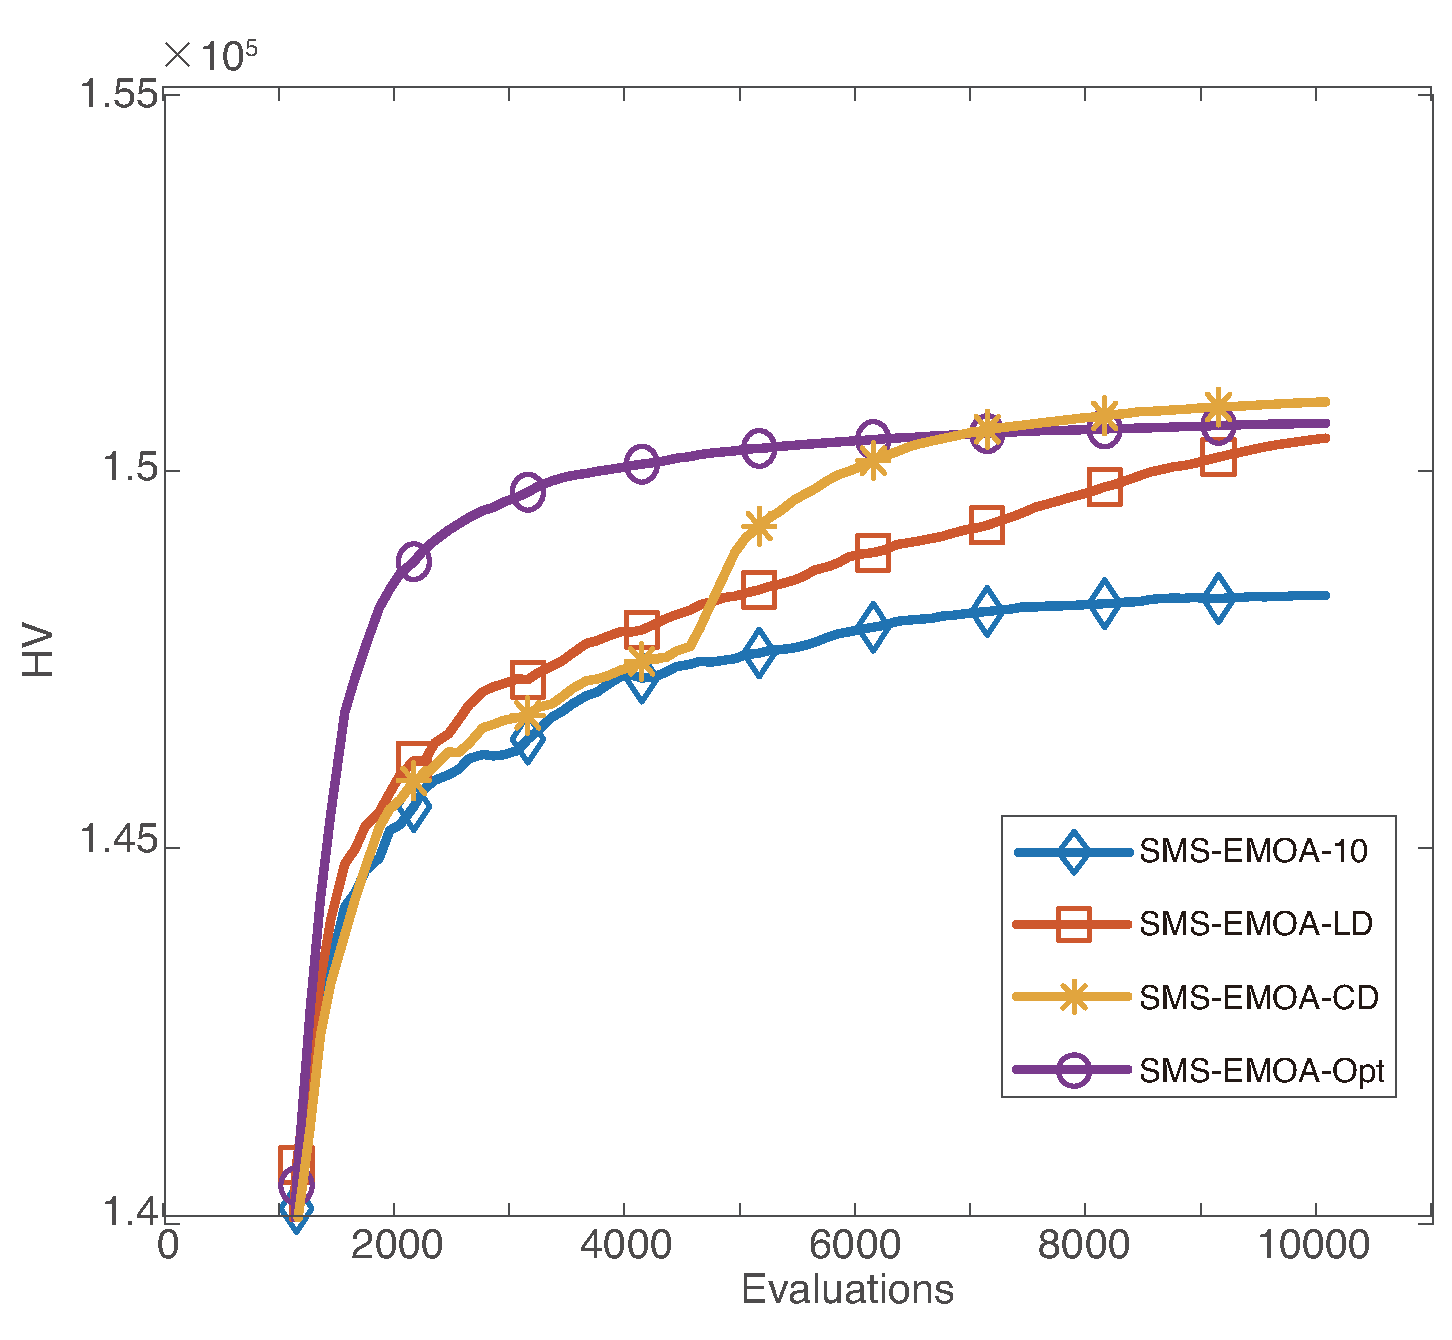
\includegraphics[width=\columnwidth]{SMSEMOA_MPDMP_hv_2}
  \caption{The comparison of four mechanisms. % on HV graph of solutions in each evaluation. 
  The value of each point is the average of 20 independent runs in each evaluation
  and the problem is MPDMP. 
  }
  \label{crdmp}
\end{figure}
We plot the HV graph of 4 mechanisms (as shown in Fig. \ref{crdmp}) on the 10-dimensional MPDMP problem. 
In Fig. \ref{crdmp}, the HV of SMS-EMOA-LD (the red curve) is gradually increased 
and finally reaches the same level as SMS-EMOA-Opt, as the value of $r$ is gradually decrease to $1+1/H$.
The HV of SMS-EMOA-CD (the yellow curve) firstly reaches a stable level similar to SMS-EMOA-10, 
for that their values of $r$ are both 10 before 4,500 evaluations. 
Then after reporting the convergence detection at about 4,500 evaluations, 
the value of $r$ in SMS-EMOA-CD reaches the optimal value $1+1/H$ 
and the HV increases. 
The reason is because the boundary solutions decrease, and on the other hand, the inner solutions increase. 
Finally, the HV of SMS-EMOA-CD is better than SMS-EMOA-Opt and SMS-EMOA-LD. 

% ---------------sub-------------- Computational Experiments ------------------------------------
% ----------------------------- The Importance of Dynamic Mechanism ----------------------------------
% 
% \subsection{The Importance of Using Dynamic Mechanism}
% We plot the final solutions distributions of some experiments including DTLZ4 and minus-DTLZ4 
% in 3-dimension (as shown in Fig. \ref{iudm1}) and in 5-dimension (as shown in Fig. \ref{iudm2}).
% The solutions distributions of Fig. \ref{iudm1:a} - \ref{iudm1:c} hint that 
% the FVEMOA do not have good performance on concave pareto front problems. 
% In Fig. \ref{iudm1:d}, the solutions are poor distributed comparing with Fig. \ref{iudm1:a}-\ref{iudm1:c}.
% This phenomenon is also observed in Fig. \ref{iudm2:d}.
% \begin{figure}[!t]
%   \centering
%   \subfloat[FV-EMOA-2]{\label{iudm1:a}
%     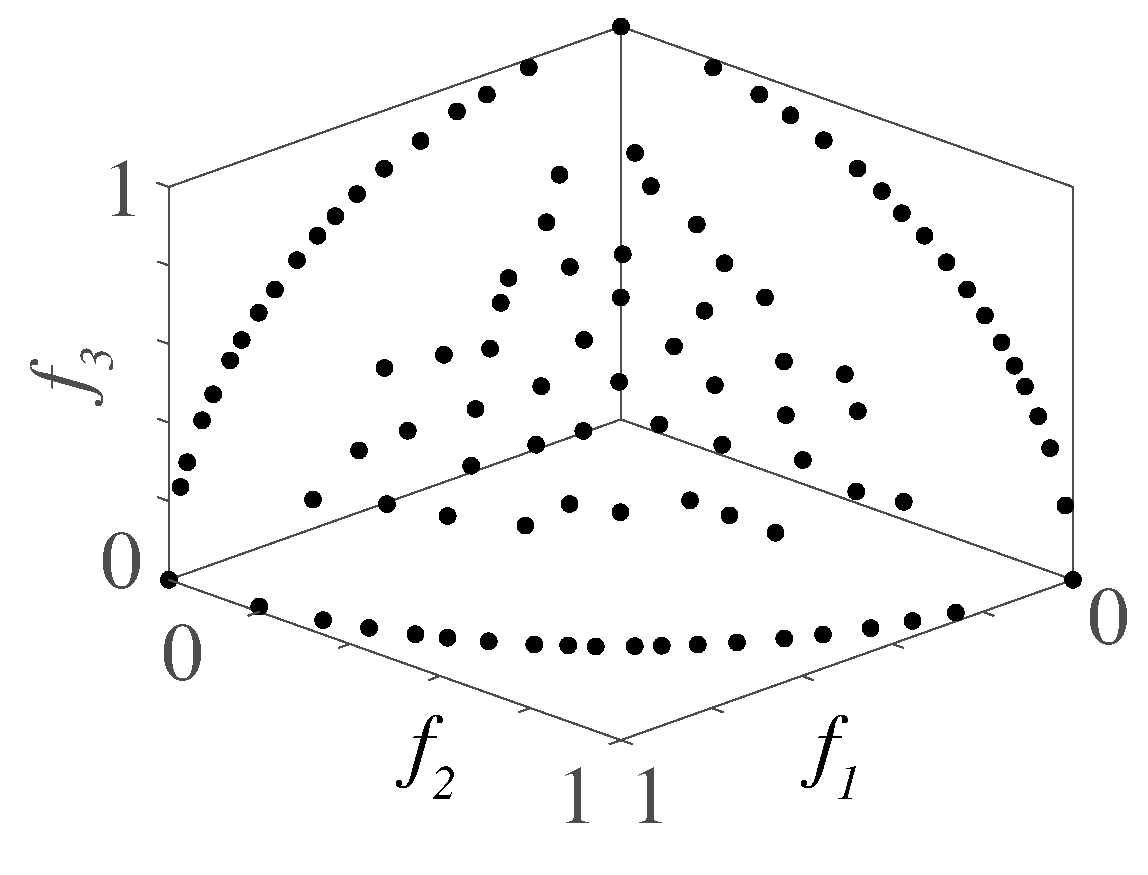
\includegraphics[width=1.5in]{FVEMOA_DTLZ4_3}}\quad
%   \subfloat[FV-EMOA-LD]{\label{iudm1:b}
%     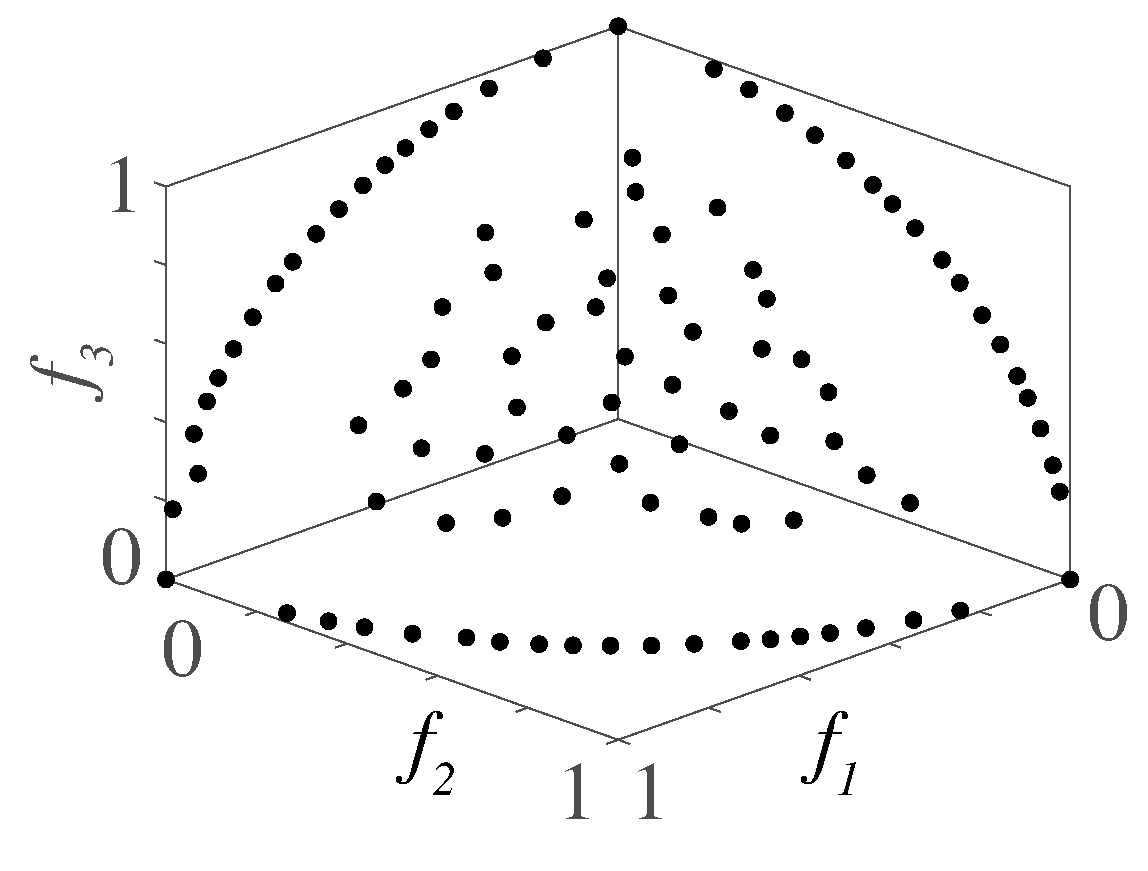
\includegraphics[width=1.5in]{FVEMOA_DR_DTLZ4_3}}\\
%   \subfloat[FV-EMOA-CD]{\label{iudm1:c}
%     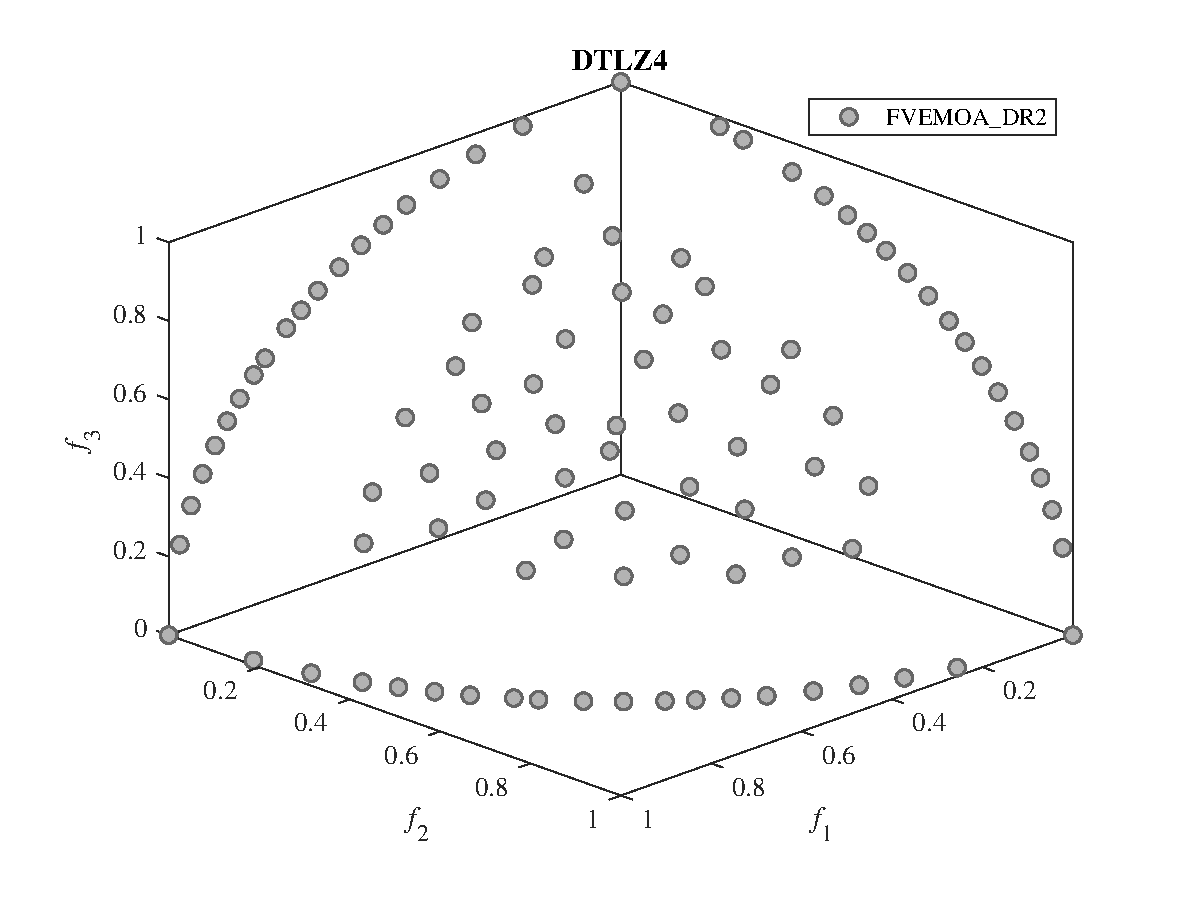
\includegraphics[width=1.5in]{FVEMOA_DR2_DTLZ4_3}}\quad
%   \subfloat[FV-EMOA-Opt]{\label{iudm1:d}
%     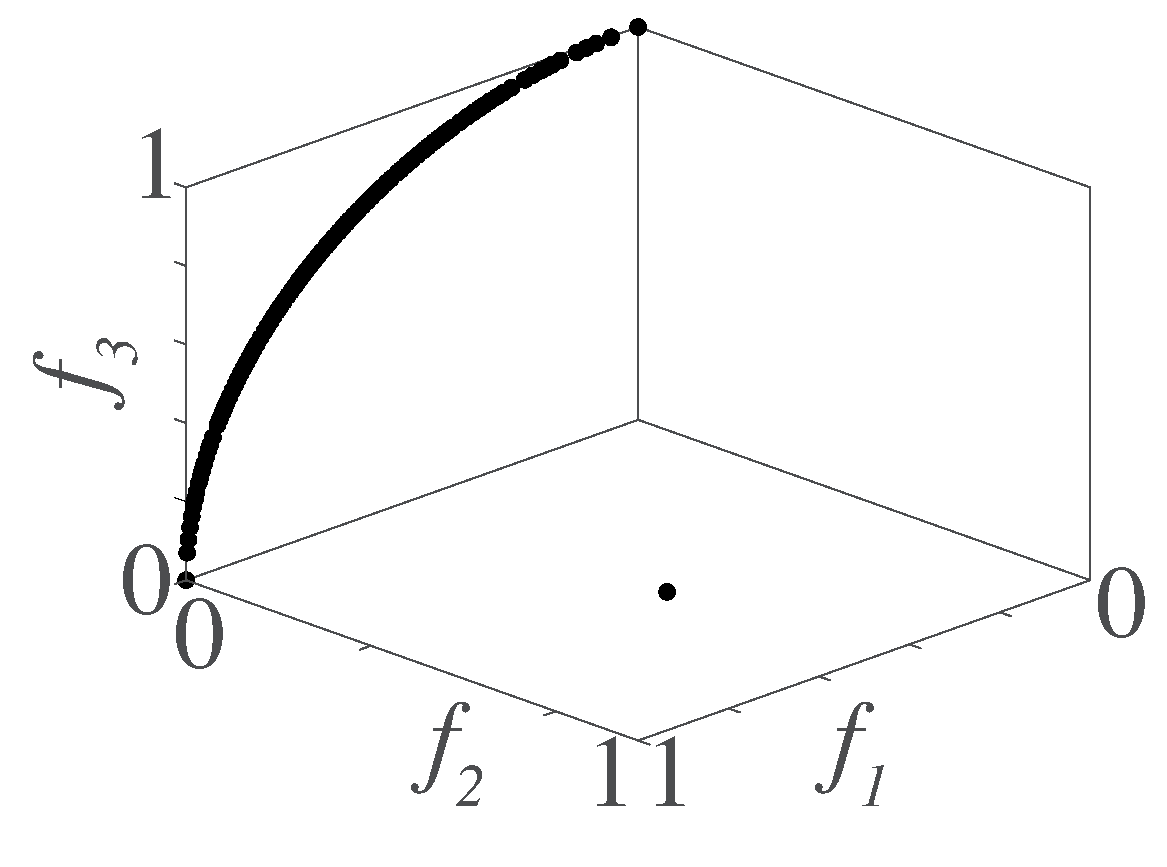
\includegraphics[width=1.5in]{FVEMOA_optimal_DTLZ4_3}}\\
%   \caption{
%     The final distribution of 4 reference point strategies on 3-dimensional DTLZ4 problems.
%   }
%   \label{iudm1}
% \end{figure} 
% \begin{figure}[!t]
%   \centering
%   \subfloat[FV-EMOA-2]{\label{iudm2:a}
%     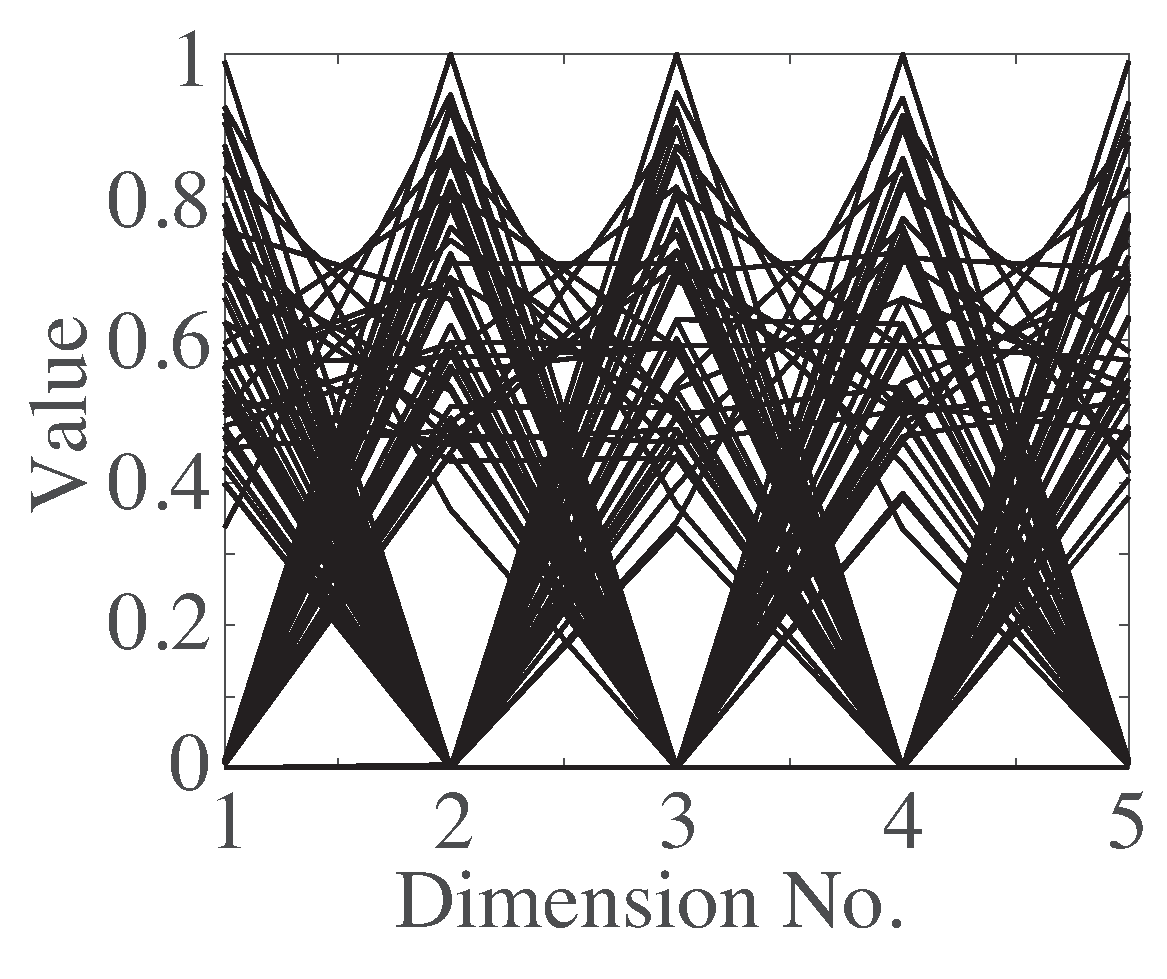
\includegraphics[width=1.5in]{FVEMOA_DTLZ4_5}}\quad
%   \subfloat[FV-EMOA-LD]{\label{iudm2:b}
%     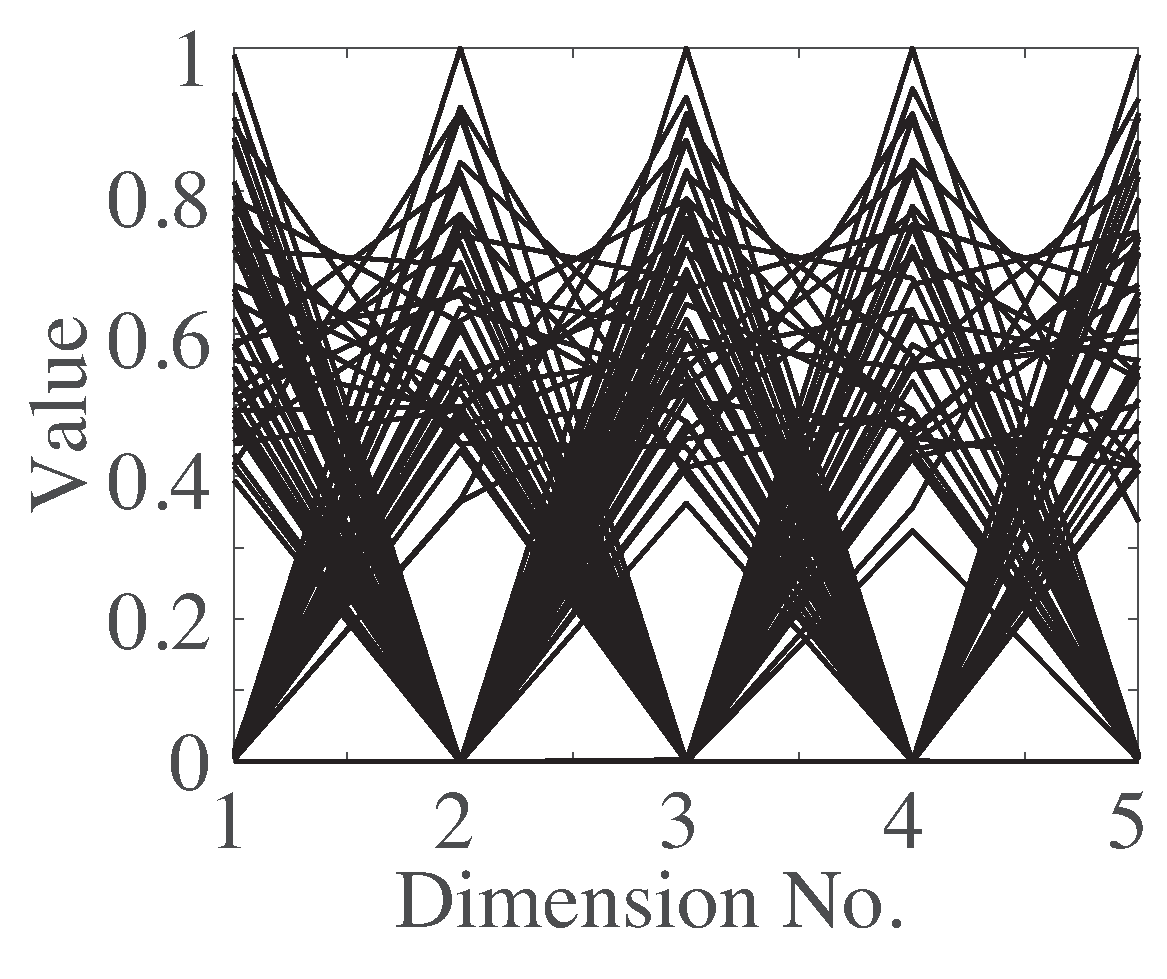
\includegraphics[width=1.5in]{FVEMOA_DR_DTLZ4_5}}\\
%   \subfloat[FV-EMOA-CD]{\label{iudm2:c}
%     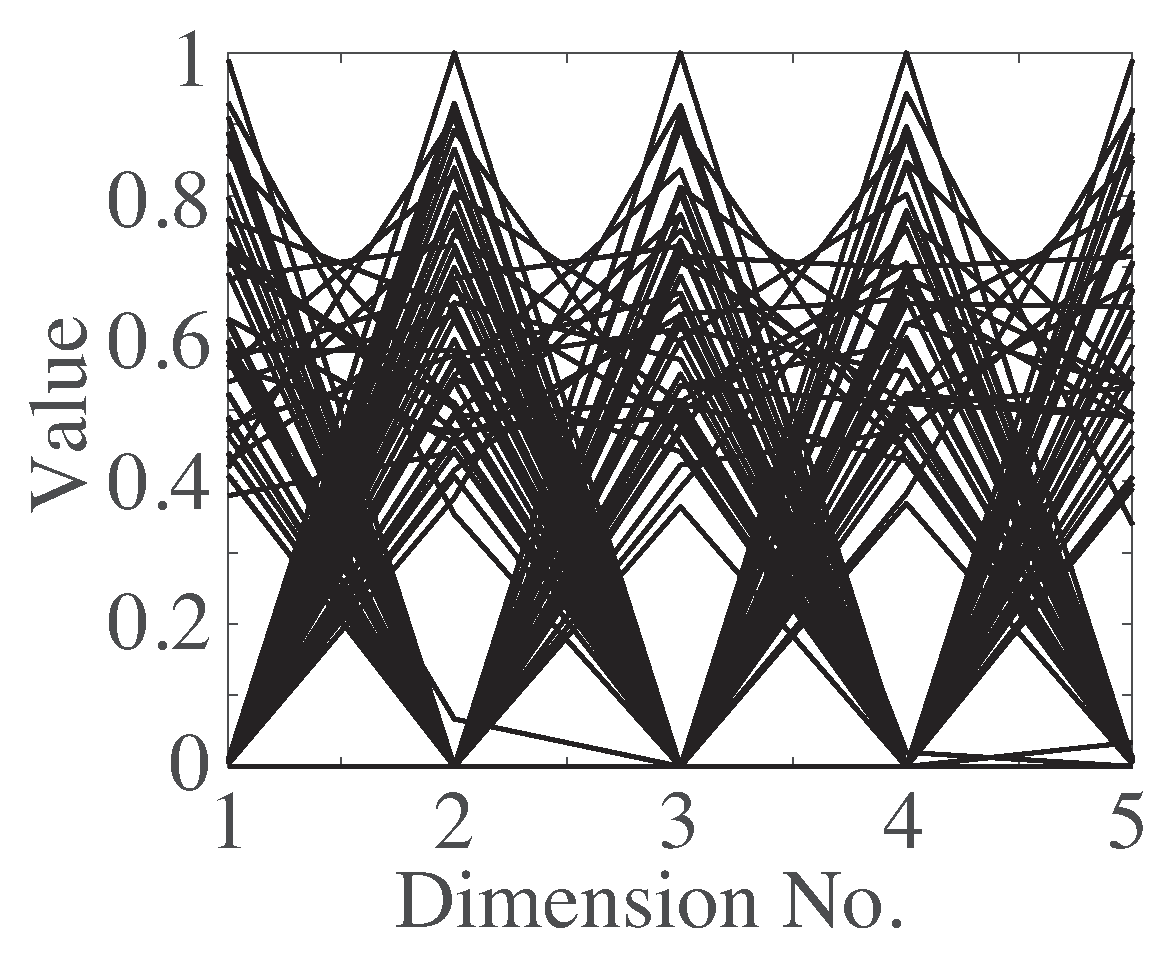
\includegraphics[width=1.5in]{FVEMOA_DR2_DTLZ4_5}}\quad
%   \subfloat[FV-EMOA-Opt]{\label{iudm2:d}
%     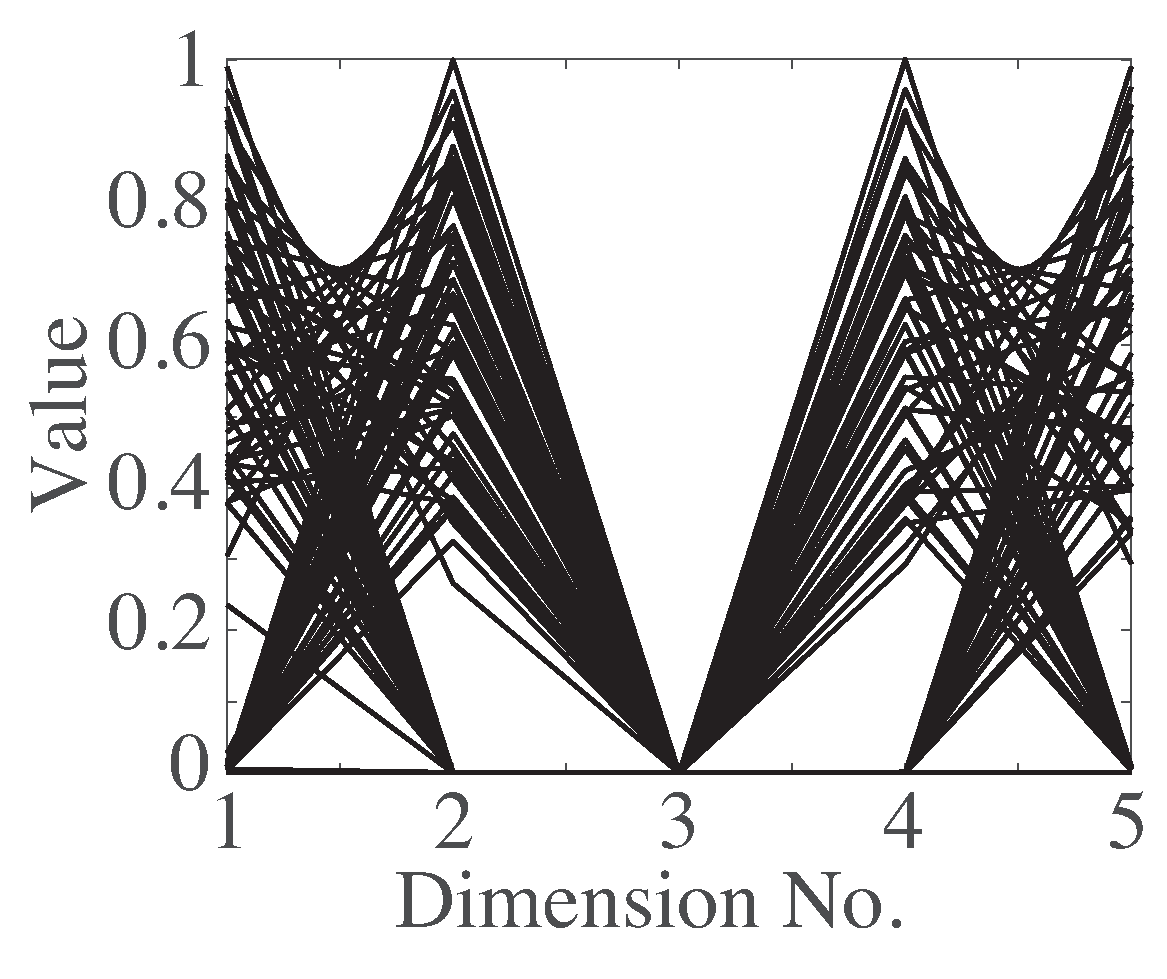
\includegraphics[width=1.5in]{FVEMOA_optimal_DTLZ4_5}}\\
%   \caption{
%     The final distribution of 4 reference point strategies on 5-dimensional DTLZ4 problems.
%   }
%   \label{iudm2}
% \end{figure} 
% The standard deviations of FV-EMOA-Opt on the DTLZ4 problem (shown in the TABLE \ref{table_tri}) are both higher
% than other three algorithms in 3- and 5-dimension($2.14e-1$  comparing with $1.21e-1, 1.31e-1, 1.76e-1$ in 3-dimension 
% and $1.01e-1$ comparing with $9.98e-2, 7.21e-2, 6.05e-2$ in 5-dimension).
% This observation also shows that the solutions distributions of some runs in FV-EMOA-Opt are poor over the total 20 runs.

% In FV-EMOA-Opt, the algorithm applies $r_{Initial} = 1+1/H$ mechanism at the early stage of algorithm 
% while other three algorithms apply $r_{Initial} = 2$.
% Even though the $r_{final}$ of FV-EMOA-LD, FV-EMOA-CD and FV-EMOA-Opt are all equal to $1+1/H$, 
% FV-EMOA-Opt can not jump out from the local minimum and estimate the pareto front well 
% due to the pool searching behavior at the early stage. 

% The above examples clearly show the importance of using dynamic mechanism, 
% that a slightly larger $r$ than $1+1/H$ can make the algorithm with a better searching behavior in 
% convergence stage where the solutions have not reached to the pareto front 
% especially for the problems which are difficult to find the whole solutions space like the DTLZ4 problem. 

% ---------------sub-------------- Computational Experiments ------------------------------------
% ----------------------------- comparison of two dynamic mechanisms ----------------------------------
% 2种机制比较
% 当evaluation足够的时候,差不多
% feasible region 大, evaluation不太够时但过了convergence点时 我的好
% rinit = 10
%
% \subsection{Comparison of Two Dynamic Mechanisms}
% We want to further investigate the differences between two dynamic mechanisms 
% (the linearly decrease mechanism and the weak convergence detection mechanism). 
% Here are the examples of the final distribution on the MaF1 problem(as shown in Fig. \ref{ctdm}).
% The total evaluation number is set to $3500$ and the convergence is detected at $3400$ evaluations. 
% The solutions distribution of FV-EMOA-CD(Fig. \ref{ctdm:c}) is similar to 
% the that of FV-EMOA-Opt(Fig. \ref{ctdm:d})
% while there are still overmany solutions on the boundary of pareto front in FV-EMOA-LD(Fig. \ref{ctdm:b}). 

% The reason is quite intuitionistic.
% In the linearly decrease mechanism, the total evaluation number is so small that it is too late for the solutions 
% to distribute evenly when reaching to the final generation. 
% But in the weak convergence detection mechanism, a convergence is reported after 3400 evaluations and 
% the algorithm still has 100 evaluations to make a good solutions distribution. 
% % conclusion里写
% \begin{figure}[!t]
%   \centering
%   \subfloat[FV-EMOA-2]{\label{ctdm:a}
%     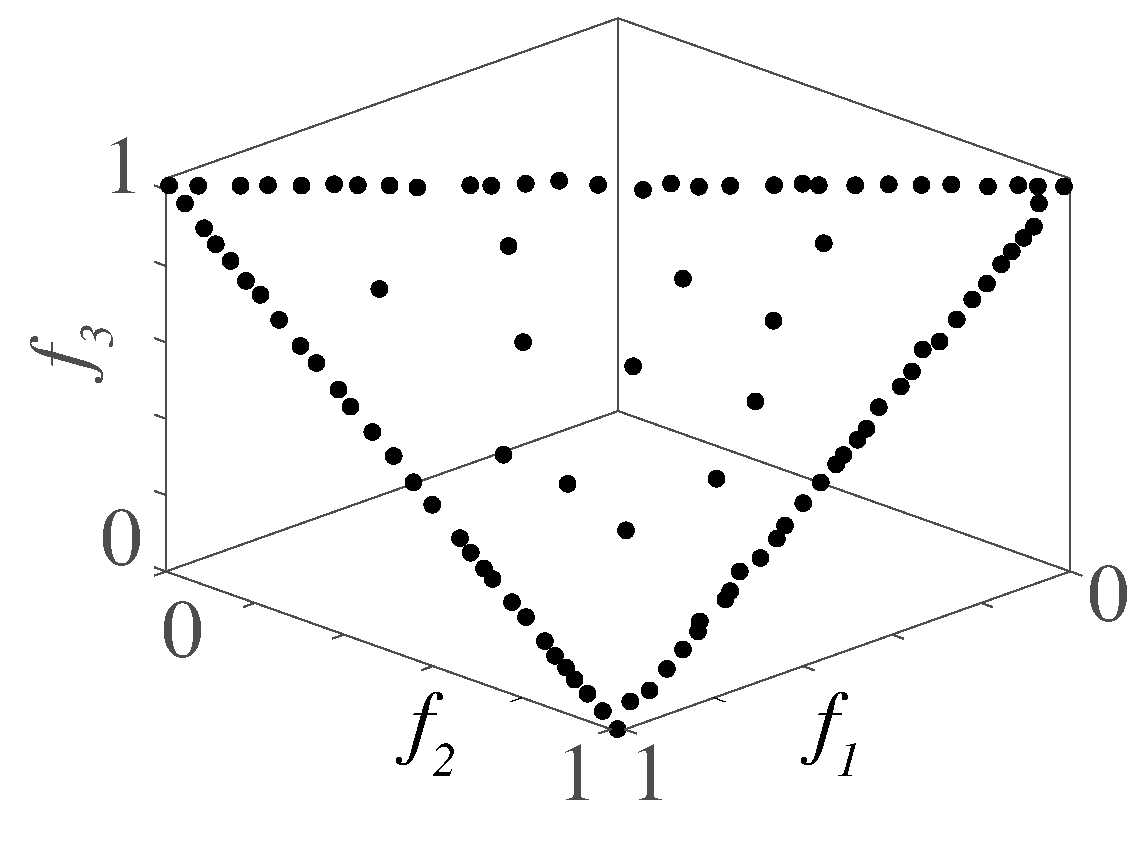
\includegraphics[width=1.5in]{FVEMOA_MaF1_M3_3500_3400convergence}}\quad
%   \subfloat[FV-EMOA-LD]{\label{ctdm:b}
%     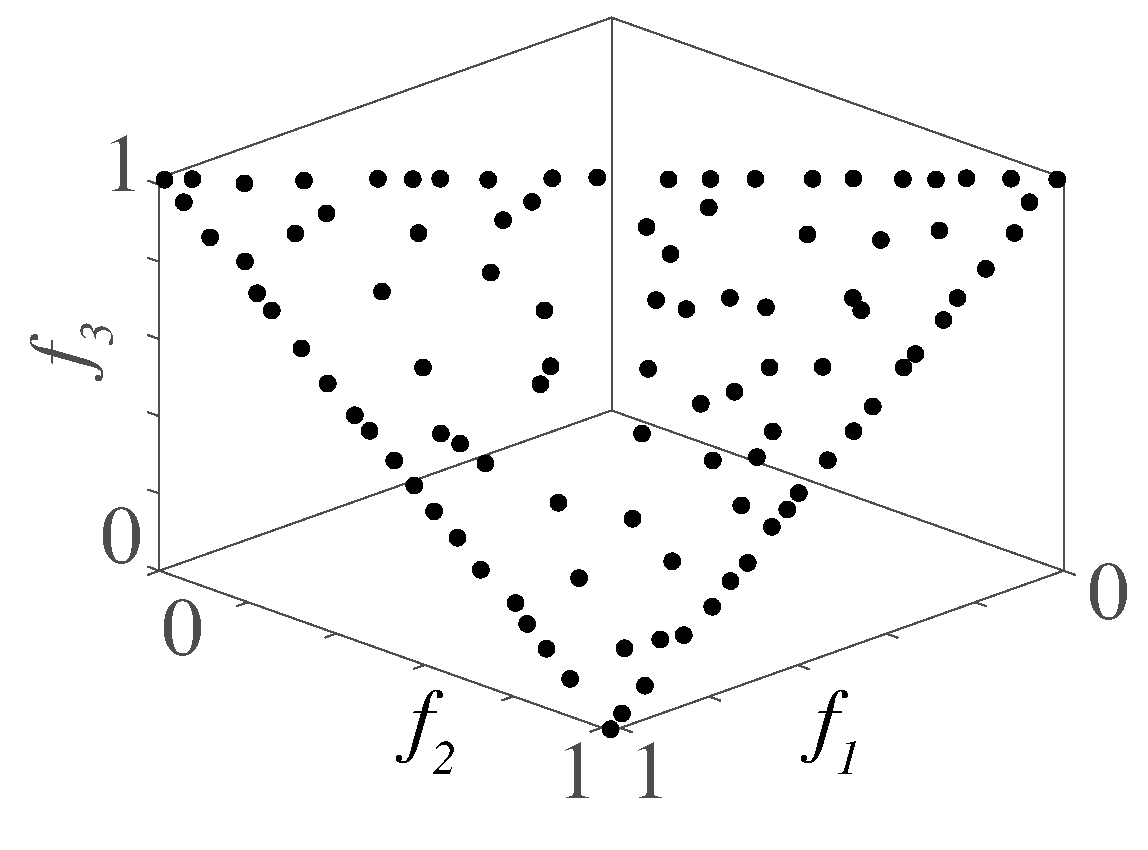
\includegraphics[width=1.5in]{FVEMOA_DR_MaF1_M3_3500_3400convergence}}\\
%   \subfloat[FV-EMOA-CD]{\label{ctdm:c}
%     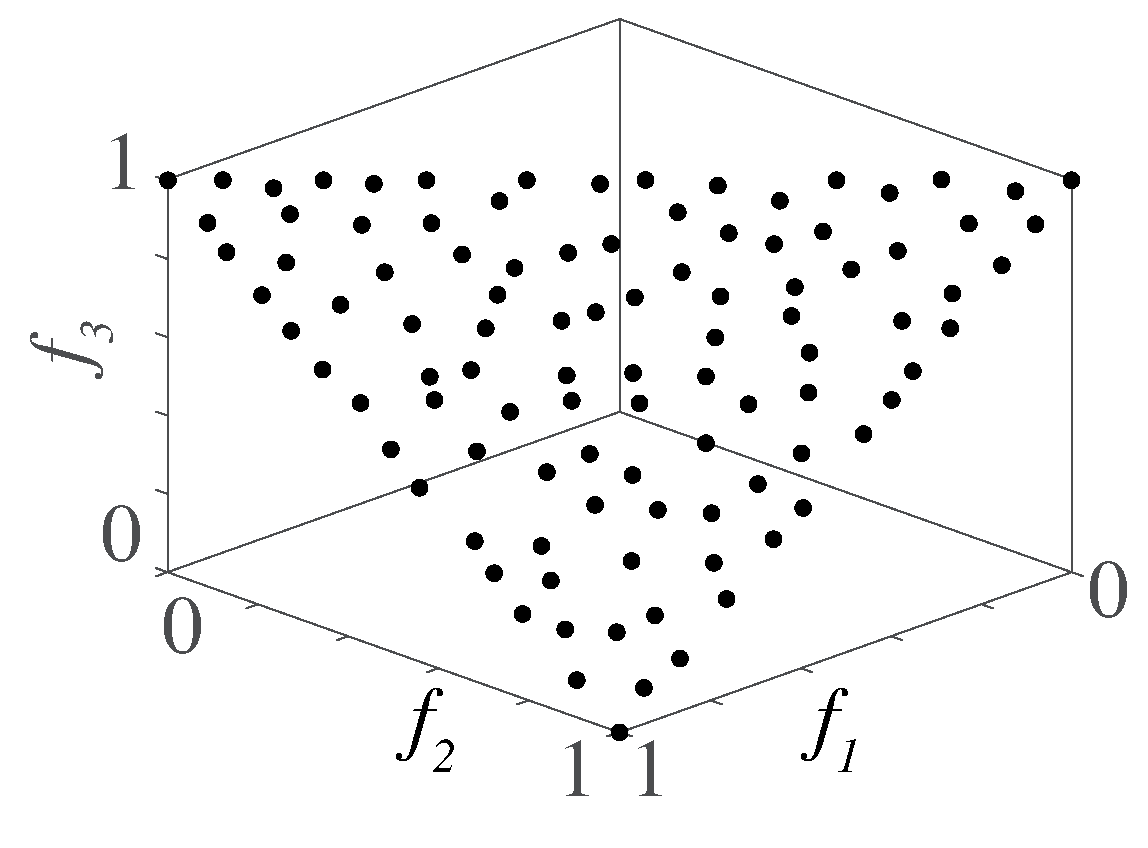
\includegraphics[width=1.5in]{FVEMOA_DR2_MaF1_M3_3500_3400convergence}}\quad
%   \subfloat[FV-EMOA-Opt]{\label{ctdm:d}
%     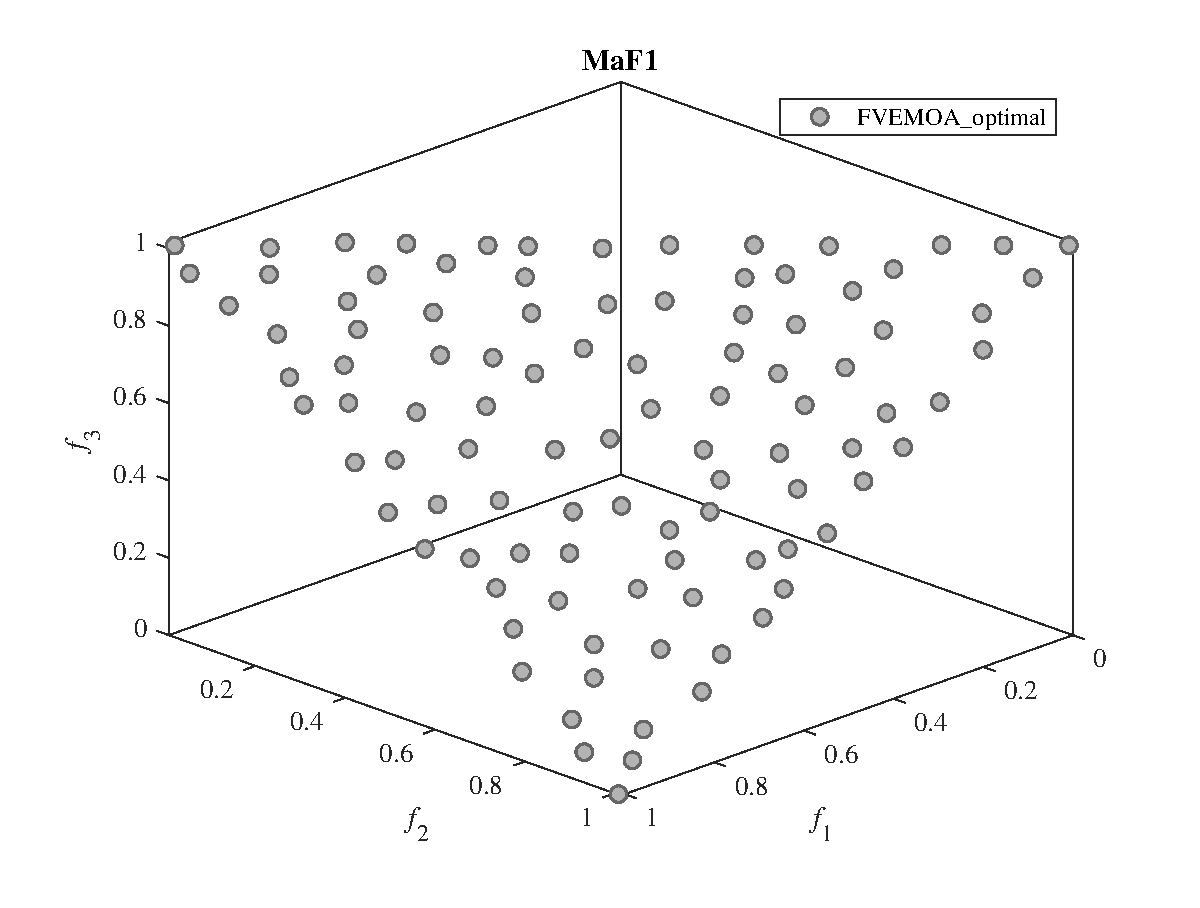
\includegraphics[width=1.5in]{FVEMOA_optimal_MaF1_M3_3500_3400convergence}}\\
%   \caption{
%     The final distribution of 4 reference point strategies on the MaF1 problem.
%     The results are obtained after $3500$ evaluations($t_{Converged} = 3400$).
%   }
%   \label{ctdm}
% \end{figure} 

\section{Conclusions}
In this paper, we emphasize the importance of reference point specification  
in SMS-EMOA by a simple example. 
Without a good reference point specification mechanism, the diversity of the final solutions will be poor
on inverted-shape PF problems. 
This phenomenon will not be observed on the triangular PF problems when the reference point is worse than the nadir point. 
Then we state the dynamic reference point specification mechanism with the illustration by two aspects:
\subsubsection{Better Searching Behavior} In the early stage, 
the solutions may not be close to the true PF. 
A larger value of $r$ can achieve a better searching behavior.
We give an example of the DTLZ2 problem. 
\subsubsection{Uniform Distribution} Considering the linear triangular problems, 
the optimal setting of reference point is $r=1+1/H$. 

We summarize the whole process of dynamic reference point specification mechanism as that,
the value of $r$ should be specified larger than $1+1/H$ at first and be equal to $1+1/H$ in the end,
as in Eqs. (\ref{f2})-(\ref{endm1}).

After that, a new dynamic reference point adaptation mechanism is proposed in this paper.
A weak convergence detection mechanism is used. 
We apply our new dynamic mechanism on different test problems including the triangular and the inverted-triangular PFs problems. 
The results show that SMS-EMOA with $r=1+1/H$ performs the worst on the problems with triangular PF, 
and SMS-EMOA with $r=10$ performs the worst on the problems with inverted-triangular PFs,
which hint the superiority of dynamic mechanism. 
SMS-EMOA with weak convergence detection mechanism performs better or worse than SMS-EMOA with linearly decrease mechanism.

We compare our new mechanism with the proposed linearly decreasing mechanism and find that
on some problems, specifically the multi-objective distance minimization problems,  
our weak convergence detection mechanism outperforms the linear decreasing mechanism. 

In the future, we plan to further investigate the behavior of our new mechanism. 
A larger dimensionality of MaOPs should be considered 
and the problems with different PF shapes should be tested and analyzed detailedly. 
Our weak convergence detection mechanism can also be further improved. 

\bibliographystyle{IEEEtran} 
\bibliography{mybibtex} 

\end{document}


